\documentclass[11pt,a4paper]{article}

\usepackage[T1]{fontenc}
\usepackage[czech]{babel}

\usepackage{amsmath}
\usepackage{amsfonts}
\usepackage{amssymb}
\usepackage{graphicx}
\usepackage[left=2cm,right=2cm,top=2cm,bottom=3.5cm]{geometry}
\usepackage{hyperref}
\usepackage{url}
\usepackage{url}
\usepackage[]{algorithm2e}
\usepackage[toc,page]{appendix}

% Colors
% ********************************************************************
\PassOptionsToPackage{dvipsnames}{xcolor}
\RequirePackage{xcolor} % [dvipsnames] 
\definecolor{halfgray}{gray}{0.55} % chapter numbers will be semi transparent .5 .55 .6 .0
\definecolor{webgreen}{rgb}{0,.5,0}
\definecolor{webbrown}{rgb}{.6,0,0}
\definecolor{Maroon}{cmyk}{0, 0.87, 0.68, 0.32}
\definecolor{RoyalBlue}{cmyk}{1, 0.50, 0, 0}
\definecolor{Black}{cmyk}{0, 0, 0, 0}


\hypersetup
{
bookmarksopen=true,
pdftitle="libGeoReport",
pdfauthor="Michal ELIAS",
pdfsubject="coordinate transformations",
pdftoolbar=true, % toolbar hidden
pdfmenubar=true, %menubar shown
pdfhighlight=/O, %effect of clicking on a link
colorlinks=true, %couleurs sur les liens hypertextes
pdfpagemode=None, %aucun mode de page
pdfpagelayout=SinglePage, %ouverture en simple page
pdffitwindow=true, %pages ouvertes entierement dans toute la fenetre
linkcolor=linkcol, %couleur des liens hypertextes internes
citecolor=citecol, %couleur des liens pour les citations
%urlcolor=linkcol %couleur des liens pour les url
colorlinks=true, breaklinks=true, bookmarks=true,bookmarksnumbered,
urlcolor=webbrown, linkcolor=RoyalBlue, citecolor=webgreen, % Link colors
}

\usepackage{fancyhdr} 
\pagestyle{fancy}
\fancyhf{}
\renewcommand{\headrulewidth}{0pt} % customise the layout...
\chead{ERA PROPRIETARY – NOT FOR DISTRIBUTION}\lhead{}\rhead{}
\cfoot{ERA PROPRIETARY – NOT FOR DISTRIBUTION}\lfoot{}\rfoot{}

\renewcommand{\contentsname}{Obsah}

\title{\normalfont{Popis souřadnicových systémů a transformace mezi vybranými systémy}}
\author{\textsc{Michal Eliaš}}
\date{}

\begin{document}

\maketitle

\setcounter{tocdepth}{2} 


% Tabulka zmien dokumentu
\begin{table}[ht!]
\centering
\begin{tabular}{c|c|c|c}
\hline
Verze & Dátum & Autor & Opis zmen \\
\hline
\hline
[0.1] & 2023-03-08 & mel & Založenie súboru\\
\hline

\end{tabular}
\end{table}

\tableofcontents % Print the table of contents

\listoffigures % Print the list of figures

\listoftables % Print the list of tables

\section*{Abstrakt}
\textit{
Dokument obsahuje kompletnú správu týkajúcu sa vývoja modelu strát. Obsahoj je jednak matematický opis modelu, potom aj konkrétne príklady. Report obsahuje porovnanie so stávajúcim modelom a diskutuje o možných vylepšeniach.
}

\newpage 
\section*{Přehled důležitějších zkratek}

\begin{table}[ht!]
  \begin{tabular}{c c l}
    CTP  & - & Conventional Terrestrial Pole  \\
    ECEF & - & Earth-Centered Earth-Fixed. Pravouhlý souřadnicový systém \\
  & - & \\   
    IERS & - & International Erath Rotation Service \\
  \end{tabular}
\end{table}
\section*{Přehled důležitějších symbolů}

\begin{table}[ht!]
  \begin{tabular}{c c l}
    TBA  & - & TBA  \\
  \end{tabular}
\end{table}
\section{Úvod}

Dokument obsahuje základní popis transformací mezi vybranými souřadný systémy. Konkrétně se jedná o tyto souřadné soustavy:

\begin{enumerate}
\item ECEF (Earth Centred Earth Fixed) je pravoúhlá geocentrická souřadnicová soustava.
\item ENU (East North Up) je pravoúhlá lokální souřadnicová soustava.
\item GEOD je soustava geodetických/elipsoidickou souřadnic definovaných na rotačním elipsoidu, např. WGS-84.
\item SPHERE je soustava sférických souřadníc
\end{enumerate}


\subsection{Rešerš literatúry}

\subsubsection{Obecná četba}

TBA

\subsubsection{Zajímavé odkazy na literatúru ve vztahu k transformacím}

TBA
\section{Poznámky}

\subsection{Transformace}

Definujme si zápis transformační matice ze souřadného systému UVW do souřadného systému XYZ například ve tvaru $\mathbf{C}_{XYZ}^{UVW}$ \cite{Grewal2001}.

Dále, ať vektor $\mathbf{v}$ obsahuje souřadnice systému XYZ, t.j. $\mathbf{v} = \left[v_{x}, v_{y}, v_{z}\right]^{T}$ a ten stejný vektor $\mathbf{v}$ ať obsahuje souřadnice $\mathbf{v} = \left[v_{u}, v_{v}, v_{w}\right]^{T}$ systému UVW. Pak pre obecný zápis transformace platí tento předpis

\begin{equation}
\begin{bmatrix}
v_{x} \\
v_{y} \\
v_{z}
\end{bmatrix} = \mathbf{C}^{UVW}_{XYZ}
\begin{bmatrix}
v_{u} \\
v_{v} \\
v_{w}
\end{bmatrix}
\label{rov:transGeneral}
\end{equation}
Systémy \textit{XYZ}, respektive \textit{UVW} reprezentují trojdimenzionální kartézské souřadné systémy.

Komponenty vektorů v jakémkoli souřadnícovém systému lze vyjádřit pomocí jejich jednotkových vektorů rovnoběžných s jejich příslušnými souřadnicovými osami. Například, ať souřadnicové osy systému XYZ označíme X, Y a Z a souřadnicové osy systému UVW označíme U, V a W, potom vektor \textbf{v} můžeme vyjádřit ve tvaru

\begin{eqnarray}
\mathbf{v} &=& v_{x}\mathbf{1}_{x} + v_{y}\mathbf{1}_{y} + v_{z}\mathbf{1}_{z} \\ \nonumber
           &=& v_{u}\mathbf{1}_{u} + v_{v}\mathbf{1}_{v} + v_{w}\mathbf{1}_{w}, 
\end{eqnarray}
kde
\begin{itemize}
\item jednotkové vektory $\mathbf{1}_{x}, \mathbf{1}_{y}, \mathbf{1}_{z}$ jsou definovány podél souřadných os X, Y a Z systému XYZ,
\item skaláry $v_{x}, v_{y}, v_{z}$ jsou komponenty vektoru \textbf{v} definovány podél souřadných os X, Y a Z systému XYZ,
\item jednotkové vektory $\mathbf{1}_{u}, \mathbf{1}_{v}, \mathbf{1}_{w}$ jsou definovány podél souřadných os U, V a W systému UVW, 
\item skaláry $v_{u}, v_{v}, v_{w}$ jsou komponenty vektoru \textbf{v} definovány podél souřadných os U, V a W systému UVW. 
\end{itemize}

Příslušné komponenty vektoru lze vyjádřit pomocí skalárního součinu příslušných jednotkových vektorů, například ve tvaru

\begin{eqnarray}
v_{x} &=& \mathbf{1}^{T}_{x}\mathbf{v} = v_{u}\mathbf{1}^{T}_{x}\mathbf{1}_{u} + v_{v}\mathbf{1}^{T}_{x}\mathbf{1}_{v} + v_{w}\mathbf{1}^{T}_{x}\mathbf{1}_{w}, \\
v_{y} &=& \mathbf{1}^{T}_{y}\mathbf{v} = v_{u}\mathbf{1}^{T}_{y}\mathbf{1}_{u} + v_{v}\mathbf{1}^{T}_{y}\mathbf{1}_{v} + v_{w}\mathbf{1}^{T}_{y}\mathbf{1}_{w}, \\
v_{z} &=& \mathbf{1}^{T}_{z}\mathbf{v} = v_{u}\mathbf{1}^{T}_{z}\mathbf{1}_{u} + v_{v}\mathbf{1}^{T}_{z}\mathbf{1}_{v} + v_{w}\mathbf{1}^{T}_{z}\mathbf{1}_{w},
\end{eqnarray}
a v maticové formě předchozí rovnice nabývají tento zápis

\begin{equation}
\begin{bmatrix}
v_{x} \\
v_{y} \\
v_{z}
\end{bmatrix} =
\begin{bmatrix}
\mathbf{1}_{x}^{T}\mathbf{1}_{u} & \mathbf{1}_{x}^{T}\mathbf{1}_{v} & \mathbf{1}_{x}^{T}\mathbf{1}_{w} \\
\mathbf{1}_{y}^{T}\mathbf{1}_{u} & \mathbf{1}_{y}^{T}\mathbf{1}_{v} & \mathbf{1}_{y}^{T}\mathbf{1}_{w} \\
\mathbf{1}_{z}^{T}\mathbf{1}_{u} & \mathbf{1}_{z}^{T}\mathbf{1}_{v} & \mathbf{1}_{z}^{T}\mathbf{1}_{w} 
\end{bmatrix} 
\begin{bmatrix}
v_{u} \\
v_{v} \\
v_{w}
\end{bmatrix} = \mathbf{C}^{UVW}_{XYZ}
\begin{bmatrix}
v_{u} \\
v_{v} \\
v_{w}
\end{bmatrix}.
\label{rov:transGeneral}
\end{equation}

Tímto jsme si odvodili souřadnicovou transformační matici $\mathbf{C}_{XYZ}^{UVW}$. Skalární součin jednotkových ortogonálních vektorů umožňuje odvodit směrové kosiny, přičemž obecně platí, že

\begin{equation}
\mathbf{1}^{T}_{a}\mathbf{1}_{b} = \cos{\left(\theta_{a, b}\right)}.
\end{equation}
V důsledku toho, souřadnicová transformační matice může být vyjádřena ve tvaru
\begin{equation}
\mathbf{C}_{XYZ}^{UVW} = 
\begin{bmatrix}
\cos{\left(\theta_{x,u}\right)} \cos{\left(\theta_{x,v}\right)} \cos{\left(\theta_{x,w}\right)} \\
\cos{\left(\theta_{y,u}\right)} \cos{\left(\theta_{y,v}\right)} \cos{\left(\theta_{y,w}\right)} \\
\cos{\left(\theta_{z,u}\right)} \cos{\left(\theta_{z,v}\right)} \cos{\left(\theta_{z,w}\right)} 
\end{bmatrix}.
\label{rov:generRotMat}
\end{equation}
Rovnice \ref{rov:generRotMat} vyjadřuje všeobecnou rotační matici v trojrozměrném prostoru.

\subsection{Translace}

V předchozí kapitole jsme se věnovali podobnostnej transformaci mezi dvěma pravoúhlými souřadný systémy. V případě posunu (translace), počátek jedné soustavy do počátku druhé soustavy jednoznačně vyjádříme pomocí vektoru

\begin{equation}
\mathbf{r} = 
\begin{bmatrix}
\left(x-u\right) & \left(y-v\right) & \left(z-w\right)
\end{bmatrix}^{T}.
\end{equation}

\subsection{Transformace kovariančních matíc}

Cílem kapitoly je navrhnout transformaci kovariančních matic souřadnic (jejích přesností) mezi uvažovanými souřadnými systémy. Princip postupu je založen na zákoně hromadění středních chyb, viz například \cite{Kubacek2013} anebo \cite{Mikhail1976}.

Matematický zápis transformace kovarianční matice mezi vybranými systémy je tento:

\begin{equation}
\mathbf {\Sigma}_{XYZ} = \mathbf{J} \mathbf{\Sigma}_{UVW} \mathbf{J}^{T},
\label{rov:CovMat}
\end{equation}
kde
\begin{itemize}
\item $\mathbf{J}$ je Jakobi matice příslušné transformace,
\item $\mathbf{\Sigma}_{UVW}$ je kovarianční matice souřadnic resp. souřadného systému, ze kterého transformujeme a
\item $\mathbf{\Sigma}_{XYZ}$ je kovarianční matice souřadnic resp. souřadného systému, do kterého transformujeme.
\end{itemize}

Interpretaci Zákona hromadění chyb a jednotlivých matíc si ukážme na nasledujícim příkladě. Majme vektorvou funkci $f\left(X\right)$ s rozměrem \textit{p}, 

\begin{equation}
\mathbf{f}\left(X\right) = \left[f_{1}\left(X\right),f_{2}\left(X\right),\cdots , f_{p}\left(X\right) \right]^{T}
\end{equation}
a neť operátor gradient pro vektor $\mathbf{X}$ s rozměrem \textit{n} je daný v tvaru

\begin{equation}
\nabla_{X} = \left[\dfrac{\partial}{\partial X_{1}}, \dfrac{\partial}{\partial X_{2}}, \cdots, \dfrac{\partial}{\partial X_{n}}\right]^{T}.
\end{equation}
Jakobiho matice \textbf{J} příslušné transformace je pak definovaný takto:

\begin{equation}
\mathbf{J}_{X} = 
\begin{bmatrix}
\nabla_{X}\mathbf{f}_{X}^{T}
\end{bmatrix}^{T} = 
\begin{bmatrix}
f_{1}\left(X\right) \\
f_{2}\left(X\right) \\
\vdots \\
f_{p}\left(X\right)
\end{bmatrix} 
\begin{bmatrix}
\dfrac{\partial}{\partial X_{1}} & \dfrac{\partial}{\partial X_{2}} & \cdots &\dfrac{\partial}{\partial X_{n}}
\end{bmatrix} =
\begin{bmatrix}
\dfrac{\partial f_{1}}{\partial X_{1}} & \dfrac{\partial f_{1}}{\partial X_{2}} & \cdots & \dfrac{\partial f_{1}}{\partial X_{n}} \\
\dfrac{\partial f_{2}}{\partial X_{1}} & \dfrac{\partial f_{2}}{\partial X_{2}} & \cdots & \dfrac{\partial f_{2}}{\partial X_{n}} \\
\vdots & \vdots & \vdots & \vdots \\
\dfrac{\partial f_{p}}{\partial X_{1}} & \dfrac{\partial f_{p}}{\partial X_{2}} & \cdots & \dfrac{\partial f_{p}}{\partial X_{n}} \\
\end{bmatrix}.
\end{equation}

Uveďme kovarnanční matici souřadnicového systému ze kterého transformujeme, respektive obecnou kovarianční matici $ \ Sigma_ {X} $. Kovariančná matice je speciální matice jak z hlediska matematického (je symetrická či pozitivní definitná), tak z hlediska fyzikálního. Obsahuje všechny rozptyly a kovariance vstupních veličin. Obecně pro ni platí
\begin{equation}
\mathbf{\Sigma}_{X_{n\times n}} = 
\begin{bmatrix}
\sigma_{X_{1}}^{2} & \sigma_{X_{1}}\sigma_{X_{2}} & \cdots & \sigma_{X_{1}}\sigma_{X_{n}}\\
\sigma_{X_{2}}\sigma_{X_{1}} & \sigma_{X_{2}}^{2} &  \cdots & \sigma_{X_{2}}\sigma_{X_{n}}\\
\vdots & \vdots & \vdots & \vdots \\
\sigma_{X_{n}}\sigma_{X_{1}} & \sigma_{X_{n}}\sigma_{X_{2}} & \cdots & \sigma_{X_{n}}^{2} & \\
\end{bmatrix}.
\end{equation}
Zaveďme si ještě výstupní kovarianční matici, teda v našem případě kovarianční matici souřadnicového systému, do kterého chceme transformovat a to například v tvaru
\begin{equation}
\mathbf{\Sigma}_{Y_{p\times p}} = 
\begin{bmatrix}
\sigma_{Y_{1}}^{2} & \sigma_{Y_{1}}\sigma_{Y_{2}} & \cdots & \sigma_{Y_{1}}\sigma_{Y_{p}}\\
\sigma_{Y_{2}}\sigma_{Y_{1}} & \sigma_{Y_{2}}^{2} &  \cdots & \sigma_{Y_{2}}\sigma_{Y_{p}}\\
\vdots & \vdots & \vdots & \vdots \\
\sigma_{Y_{p}}\sigma_{Y_{1}} & \sigma_{Y_{p}}\sigma_{Y_{2}} & \cdots & \sigma_{Y_{p}}^{2} & \\
\end{bmatrix}.
\end{equation}

Podle rovnice \ref{rov:CovMat}, kovarianční matici v systému transformovaných souřadníc výjadříme pomocí

\begin{eqnarray}
& &
\begin{bmatrix}
\sigma_{Y_{1}}^{2} & \sigma_{Y_{1}}\sigma_{Y_{2}} & \cdots & \sigma_{Y_{1}}\sigma_{Y_{p}}\\
\sigma_{Y_{2}}\sigma_{Y_{1}} & \sigma_{Y_{2}}^{2} &  \cdots & \sigma_{Y_{2}}\sigma_{Y_{p}}\\
\vdots & \vdots & \vdots & \vdots \\
\sigma_{Y_{p}}\sigma_{Y_{1}} & \sigma_{Y_{p}}\sigma_{Y_{2}} & \cdots & \sigma_{Y_{p}}^{2} & \\
\end{bmatrix} = \\ \nonumber
& &
\begin{bmatrix}
\dfrac{\partial f_{1}}{\partial X_{1}} & \dfrac{\partial f_{1}}{\partial X_{2}} & \cdots & \dfrac{\partial f_{1}}{\partial X_{n}} \\
\dfrac{\partial f_{2}}{\partial X_{1}} & \dfrac{\partial f_{2}}{\partial X_{2}} & \cdots & \dfrac{\partial f_{2}}{\partial X_{n}} \\
\vdots & \vdots & \vdots & \vdots \\
\dfrac{\partial f_{p}}{\partial X_{1}} & \dfrac{\partial f_{p}}{\partial X_{2}} & \cdots & \dfrac{\partial f_{p}}{\partial X_{n}} \\
\end{bmatrix}
\begin{bmatrix}
\sigma_{X_{1}}^{2} & \sigma_{X_{1}}\sigma_{X_{2}} & \cdots & \sigma_{X_{1}}\sigma_{X_{n}}\\
\sigma_{X_{2}}\sigma_{X_{1}} & \sigma_{X_{2}}^{2} &  \cdots & \sigma_{X_{2}}\sigma_{X_{n}}\\
\vdots & \vdots & \vdots & \vdots \\
\sigma_{X_{n}}\sigma_{X_{1}} & \sigma_{X_{n}}\sigma_{X_{2}} & \cdots & \sigma_{X_{n}}^{2} & \\
\end{bmatrix}
\begin{bmatrix}
\dfrac{\partial f_{1}}{\partial X_{1}} & \dfrac{\partial f_{2}}{\partial X_{1}} & \cdots & \dfrac{\partial f_{p}}{\partial X_{1}} \\
\dfrac{\partial f_{1}}{\partial X_{2}} & \dfrac{\partial f_{2}}{\partial X_{2}} & \cdots & \dfrac{\partial f_{p}}{\partial X_{2}} \\
\vdots & \vdots & \vdots & \vdots \\
\dfrac{\partial f_{1}}{\partial X_{n}} & \dfrac{\partial f_{2}}{\partial X_{n}} &  \cdots & \dfrac{\partial f_{p}}{\partial X_{n}}.\\
\end{bmatrix}
\end{eqnarray}

Rozptyl veličín systému transformované soustavy souřadníc, například $\sigma_{Y_{1}}^{2}$ po přenásobení matíc v předcházejíci rovnici, je 
\begin{equation}
\sigma_{Y_{1}}^{2} = \sum_{i}\left(\dfrac{\partial f_{1}}{\partial X_{i}}\right)^{2} + {\sum\sum}_{i\neq j}\dfrac{\partial f_{1}}{\partial X_{i}}\dfrac{\partial f_{1}}{\partial X_{j}}\sigma_{X_{i}X_{j}}
\end{equation}
a kovariance mezi veličinami $X_{1}\ \textbf{a}\ X_{2}$ bude
\begin{equation}
\sigma_{X_{1}X_{2}} = \sum_{i} {\dfrac{\partial f_{1}}{\partial X_{i}}\dfrac{\partial f_{2}}{\partial X_{i}}\sigma_{X_{i}}^{2}} + {\sum\sum}_{i\neq j}\dfrac{\partial f_{1}}{\partial X_{i}}\dfrac{\partial f_{2}}{\partial X_{j}}\sigma_{X_{i}X_{j}}.
\end{equation}

\newpage
\subsection{Súradnicové systémy}


\subsubsection{ECEF - Earth Centred Earth Fixed}

\begin{figure}[ht!]
\begin{center}

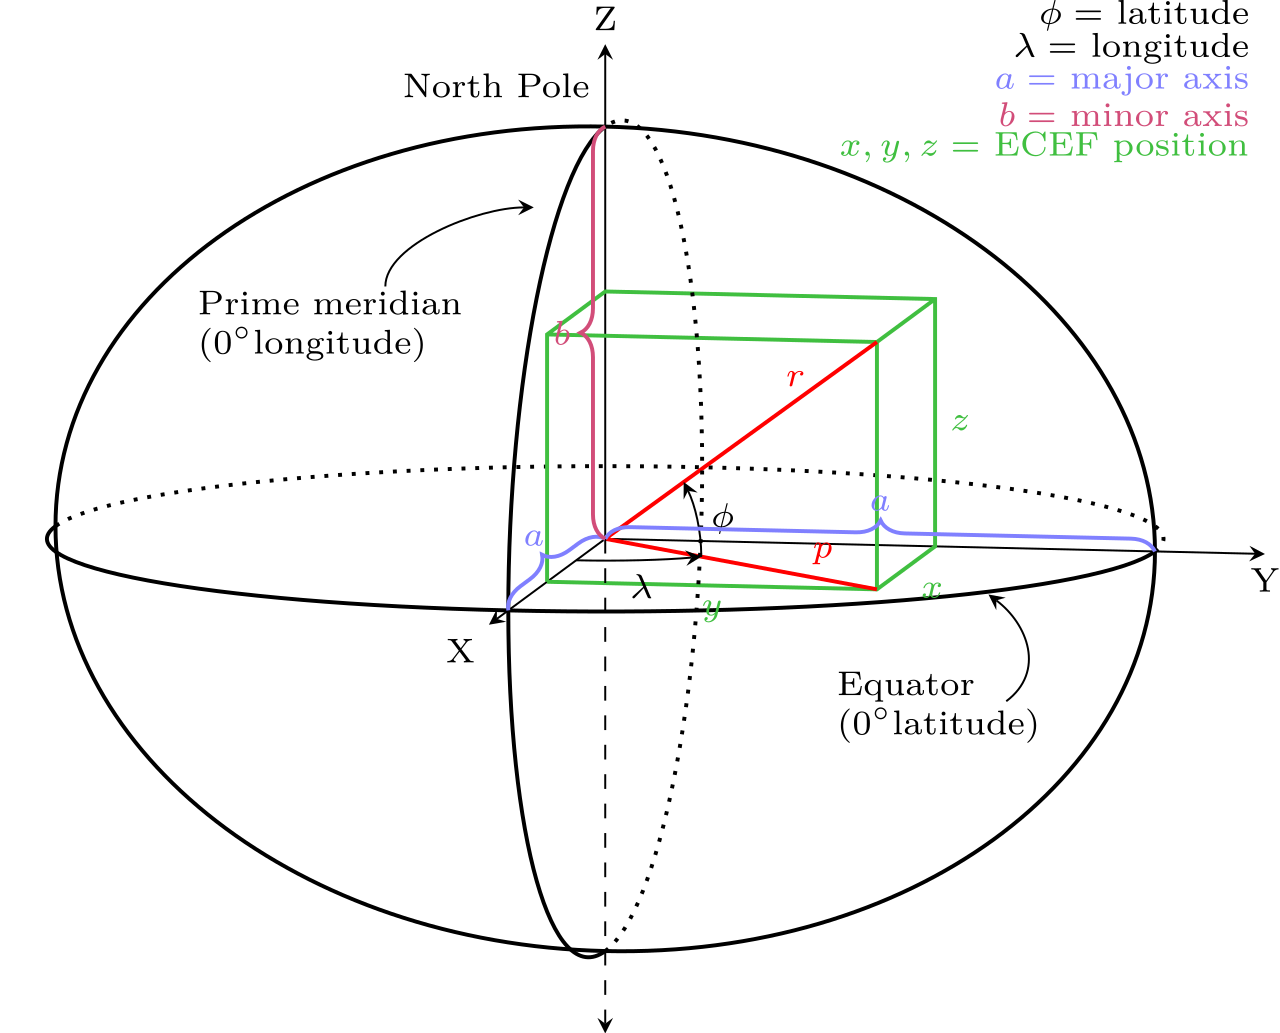
\includegraphics[width=0.60\textwidth]{FIG/ecef_wiki}
\caption{Zobrazení bodu v ECEF soustavě souřadnic. Obrázek je převzat z \cite{ecefWiki}.}
\label{fig:ecef}
\end{center}
\end{figure}

Základní kartézská pravouhlá soustava souřadníc, naúříklad tak, jako je zobrazená na obrázku \ref{fig:ecef}, je definována takto \cite{Soler1988}, \cite{Kovar2016}:

\begin{itemize}
\item počátek soustavy je soustředěn v geocentre, t.j. v gravitačním středu zemského tělesa,
\item osa \textbf{Z} směruje do místa zemského severního pólu, který je definován podle IERS. Protože poloha pólu sa v čase mění, používá se střední poloha zemského pólu (CTP).
\item osa \textbf{X} prochází bodem nulové zeměpisné délky, t.j. Greenwich poledníkem, který je definován podle IERS a míři do průsečníku tohto poledníku a roviny rovníku,
\item osa \textbf{Y} doplňuje pravotočivý pravouhlý sýstém souřadníc.
\end{itemize}

\subsubsection{ENU - East-North-Up}

Některé výpočty souřadníc je praktičtější provádět v lokální souřadnicové soustavě například vzdálenosť radarového přijímače od daného bodu atp.,\cite{Kovar2016}, \cite{Mayer2002}. ENU je lokální pravouhlá soustava souřadnic, pričemž její definice a umístnění počátku soustavy a souřadnicových os, dle značení na obrázku \ref{fig:enu}, jsou:
 
\begin{itemize}
\item počátek systému soustavy souřadníc je umiestnený v středě regiónu záujmu a to  buď na povrchu anebo blízko povrchu referenčního tělesa (elipsoid, koule),
\item osa \textbf{n} (North) směruje na sever, 
\item osa \textbf{e} (East) směruje na východ a 
\item osa \textbf{u} (Up) je totožná s normálou referenčního tělesa (elipsoid, koule). 
\end{itemize}

\begin{figure}[ht!]
\begin{center}

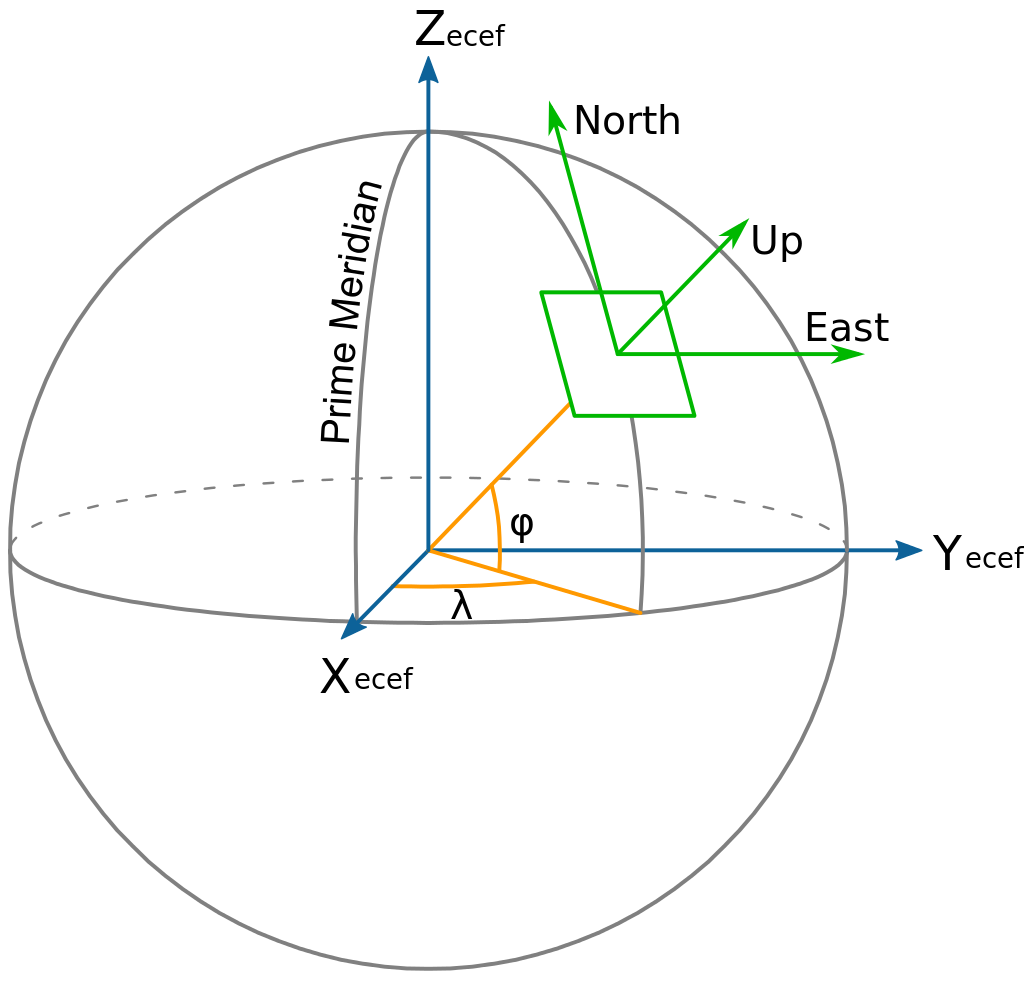
\includegraphics[width=0.50\textwidth]{FIG/enu_wiki}
\caption{Zobrazení systému souřadnic East-North-Up. Obrázek je převzat z \cite{enuWiki}.}
\label{fig:enu}
\end{center}
\end{figure}

\subsubsection{GEOD - Systém geodetických souřadníc}

\begin{figure}[ht!]
\begin{center}
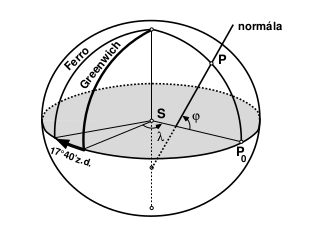
\includegraphics[width=0.50\textwidth]{FIG/geod_cimb}
\caption{Geodetické zeměpisné souřadnice. Obrázek je převzat z \cite{Cimbalnik1997}.}
\label{fig:geod}
\end{center}
\end{figure}

V praktických úlohách se poloha bodu popisuje pomocí geodetických anebo elipsoidických souřadníc. Elipsoidických proto, protože se definuje pomocí zvoleného zemského elipsoidu. Ten slouží k aproximaci fyzického zemského tělesa. Základní matematické vzorce určené pro odvození elipsoidu jsou obsahem přílohy \ref{appRefEll} a přehled konstant globálne užitých elipsoidů jsou obsahem přílohy \ref{appRefEllConst}.

Poloha bodu \textbf{P} na obrázku \ref{fig:geod} se vyjadřuje třemi souřadnicemi:

\begin{enumerate}
\item geodetickou zeměpisnou šířkou $\varphi$,
\item geodetickou zeměpisnou délkou $\lambda$,
\item geodetickou výškou.
\end{enumerate} 

Geodetická zeměpisná šířka $\varphi$ bodu \textbf{P} je uhel, který svírá normála v bodě P k povrchu elipsoidu, s rovinou rovníku. Geodetická zeměpisná délka $\lambda$ je úhel, který svírá rovina poledníku tohoto bodu s rovinou nultého poledníku. Za nultý poledník je mezinárodně volen ten, který prochází stabilizovaným bodem na astronomické observatoři v Greenwich. Geodetická výška se měří podél normály mezi referenčním elipsoidem a bodem \textbf{P}.

\subsubsection{SPHERE - Systém sférických súradníc}

Koule je základní a nejjednoduchší aproximace zemského tělesa. Sférické souřadnice tvoří systém souřdnic, které popisujou polohu bodu na sféře. Referenční koule je pak definovaná sférickým poloměrem. Pro praktické výpočty se jeho hodnota často zpočíta jako středný pomoměr křivosti (a to z důvodu zachování objemu eliposidu během jeho zobrazení na kouli, t.j. v místě lokálni aproximace - viz příloha \ref{appRefEll}).
 
\begin{figure}[ht!]
\begin{center}
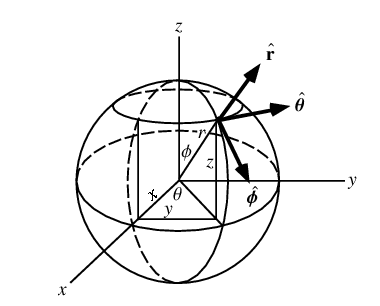
\includegraphics[width=0.50\textwidth]{FIG/sphere_wolf}
\caption{Sférické polárni souřadnice. Obrázek je převzat z \cite{sphereWolf}.}
\label{fig:sphere}
\end{center}
\end{figure}

Dle situace zobrazené na obrázku \ref{fig:sphere}, poloha bodu na sféře je vyjadřená soustavou tří souřadníc:
\begin{itemize}
\item $\theta$ hodnota azimutu v rovině rovníka. Pokud je uhel značený symbolem $\lambda$, pak poukazuje na zeměpisnou délku,
\item $\phi$ hodnota polárniho úhla počítaná od zenitu (také zenitový úhel). Pokud je uhel značený symbolem $\varphi^{'}$, pak poukazuje na doplnek zemepisej délky od zenitu, t.j. $\varphi = 90 - \varphi^{'}$ a
\item r, je středný polomer Zeme.
\end{itemize}

\newpage

\subsubsection{AES - Systém polárnych súradníc}

AES je súradný systém, ktorý pozostáva z týchto súradníc: azimut, elevačný uhol a spojnica medzi lokálnym počiatkom a cieľom. Jedná sa o systém polárnych súradníc. Lokálny počiatok súradného systému je charakterizovaný geodetickými súradnicami $lat_{0}, lon_{0}, h_{0}$. Na obrázku \ref{fig:aes} je tento systém názorne zobrazený.

\begin{figure}[ht!]
\begin{center}
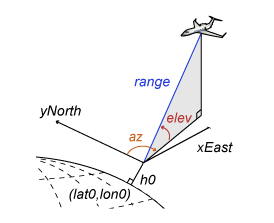
\includegraphics[width=0.50\textwidth]{FIG/AES}
\caption{Polární souřadnice. Obrázek je převzat z \cite{aesMatlab}.}
\label{fig:aes}
\end{center}
\end{figure}



\section{Transformace souřadníc a jejích kovariančních matíc medzi vybranými souřadnicovými soustavami}

\subsection{ECEF $\rightarrow$ ENU}
Předpokládejme, že v tomto příkladu je uvažovaný rotační elipsoid (například WGS-84 nebo GRS-80) geocentrický, to znamená, že střed elipsoidu se nachází ve středu zemského tělesa. Transformace souřadnic pak mezi zemským geocentrickým systémem souřadnic (xyz) a lokálním topocentrickým (nebo také lokálním geodetickým - enu) systémem může být vyjádřený předpisem \cite{Soler1998}

\begin{equation}
\begin{bmatrix}
e \\
n \\
u
\end{bmatrix} = 
\mathbf{C}_{enu}^{xyz}
\begin{bmatrix}
x \\
y \\
z
\end{bmatrix}.
\label{rov:ecef2enu1}
\end{equation}

Pro popis transformace mezi uvedenými systémy si potřebujeme odvodit transformační matici, v tomto případě takzvanou rotační matici. Vycházejme z rovnice \ref{rov:generRotMat}. Rotační matici pak zostavíme pro rotaci v prostoru a to pomocí jednoduchých rotací v každé ose samostatně.

Rotační matice kolem osy \textit{z} ve směru hodinových ručiček nabude tvar
\begin{equation}
\mathbf{R_{3}}\left(\theta\right) = 
\begin{bmatrix}
\cos{\left(\theta\right)} & \sin{\left(\theta\right)} & 0 \\
-\sin{\left(\theta\right)} & \cos{\left(\theta\right)} & 0 \\
0 & 0 & 1
\end{bmatrix},
\end{equation}
přičemž rotace kolem osy \textit{z} je $\cos{\left(\theta_{z, w} \right)} = \cos{\left(0\right)} = 1$, protože úhel mezi osama \textit{z} a \textit{w}, které jsou v tomto přikladě totožné, je roven nule. Dále platí, že kosinus úhlu $ \cos{\left(\theta_{z, u} \right)}= \cos{\left(90\right)} = 0 $, protože \textit {z} a \textit {u} jsou na sebe kolmé. Stejně tento předpoklad platí i pro $\cos{\left(\theta_{z,v}\right)}$, $\cos{\left(\theta_{x,w}\right)}$ a $\cos{\left(\theta_{y,w}\right)}$.

Analogicky postup bude platit i pro ostatní dvě rotace a tedy rotace kolem osy \textit{x} je
\begin{equation}
\mathbf{R_{1}}\left(\theta\right) = 
\begin{bmatrix}
1 & 0 & 0 \\
0 &  \cos{\left(\theta\right)} & \sin{\left(\theta\right)} \\
0 & -\sin{\left(\theta\right)} & \cos{\left(\theta\right)} \\
\end{bmatrix},
\end{equation}
a kolem osy \textit{y}
\begin{equation}
\mathbf{R_{2}}\left(\theta\right) = 
\begin{bmatrix}
\cos{\left(\theta\right)} & 0 & -\sin{\left(\theta\right)} \\
0 & 1 & 0 \\
\sin{\left(\theta\right)} & 0 & \cos{\left(\theta\right)} \\
\end{bmatrix},
\end{equation}

Vyjádření transformační matice $\mathbf {C}_{enu}^{xyz} $ mezi dvěma pravoúhlými kartézskymi souřadnicovými systémy ECEF a ENU je založen na součinu dvou rotací, konkrétně:
\begin{enumerate}
\item rotaci kolem osy \textit{z} o úhel $\pi/2 + \lambda $ a
\item rotaci kolem osy \textit{y} o úhel $\pi/2 - \varphi $,
\end{enumerate}
kde úhlové stupně $\lambda$, respektíve $\varphi$ geograficky představují stupeň otočení jedné soustavy od druhé ve směru zeměpisné délky ($\lambda$) a ve směru zeměpisné šířky ($\varphi$).

Potom transformace mezi systémy se dá vyjádřit ve tvaru

\begin{equation}
\begin{bmatrix}
e \\
n \\
u
\end{bmatrix} =
\mathbf{R_{1}}\left(\pi/2-\varphi\right)\mathbf{R_{3}}\left(\pi/2+\lambda\right)
\begin{bmatrix}
x \\
y \\
z
\end{bmatrix} =
\begin{bmatrix}
-\sin{\left(\lambda\right)} & \cos{\left(\lambda\right)} & 0 \\
-\cos{\left(\lambda\right)}\sin{\left(\varphi\right)} & -\sin{\left(\lambda\right)}\sin{\left(\varphi\right)} & \cos{\left(\varphi\right)} \\
\cos{\left(\lambda\right)}\cos{\left(\varphi\right)} & \sin{\left(\lambda\right)}\cos{\left(\varphi\right)} & \sin{\left(\varphi\right)}
\end{bmatrix}
\begin{bmatrix}
x \\
y \\
z
\end{bmatrix}.
\label{rov:ecef2enu2}
\end{equation}

Z předchozího zápisu plyne, že během rotace pravoúhlých souřadnicových soustav předpokládáme, že počátky souřadnic jsou shodné. V případě, že počátek, například soustavy ENU umístíme na povrch referenčního tělesa (elipsoid případně sféry), je zapotřebí doplnit posun mezi soustavami. Potom rovnice \ref{rov:ecef2enu2} nabude tvar

\begin{equation}
\begin{bmatrix}
e \\
n \\
u
\end{bmatrix} =
\mathbf{R}
\begin{bmatrix}
x - x_{0} \\
y - y_{0} \\
z - z_{0}
\end{bmatrix},
\label{rov:ecef2enu22}
\end{equation}

Při transformaci kovariančných matic vycházejme z předpokladu a definice Zákona hromadění středních chyb. Budeme vycházet z článku Transformace kovariančních matic. Předpokládejme, že kovariančná matice souřadnic soustavy ze které chceme transformovat $\Sigma_{xyz}$, je známá a to například jako důsledek numerického výpočtu (regrese, vyrovníní, estimace souřadnice a jejich přesností atp.). Hlavní úlohou je v tomto kroku vyčíslit Jakobiho matici. Rozepsáním matic pro jednotlivé veličiny \textit{e,n,u} z předchozích rovnic a následným parciálním derivovaním podle veličin \textit{x,y,z} snadno zjistíme, že Jakob matice $\mathbf{J}$ je totožná s rotační matici $\mathbf{R}$ a tedy
\begin{equation}
\mathbf{J} = \mathbf{R}.
\end{equation}
Kovarianční matice souřadníc systému ENU pak nadobude tvaru
\begin{equation}
\mathbf{\Sigma}_{enu} = \mathbf{J}\mathbf{\Sigma}_{xyz}\mathbf{J}^{T} = \mathbf{R}\mathbf{\Sigma}_{xyz}\mathbf{R}^{T}.
\end{equation}

\subsubsection{Příklad transformace z ECEF $\rightarrow$ ENU}

Nechť bod A je vyjádřen v souřadnicích souřadného systému ECEF a hodnoty souřadnic jsou:
\begin{itemize}
\item $x = 4198944.6161$ m
\item $y = 174747.2383$ m
\item $z = 4781886.8769$ m
\end{itemize}

Mějme bod B, jehož geodetické souřadnice jsou $ \varphi = 48.8862 deg$, $\lambda = 2.3343 deg$ a geodetická výška je $ h = 174.5217 m $. Úhlové souřadnice použijeme jednak k natočení souřadných soustav (viz rotační matice v rovnici \ref{rov:ecef2enu2}) a společně se zadanou elipsoidickou výškou, k umístění počátku ENU soustavy, který umístíme nad povrch rotačního elipsoidu. Úkolem je vyjádřit souřadnice bodu \textit{A} v soustavě ENU a s přihlédnutím definovaného počátku ENU soustavy v bodě B.

Vektor pravoúhlých souřadnic bodu B, tj $ \left(x_{0}, y_{0}, z_{0} \right)$ získáme transformací GEOD2ECEF(). ENU souřadnice bodu A s přihlédnutím k umístění počátku ENU soustavy v bodě B a vypočítané podle \ref{rov:ecef2enu22}, jsou:
\begin{itemize}
\item $e = 3579.4232 $ m
\item $n = -688.3514 $ m
\item $u = -51.0524 $ m.
\end{itemize}

Pseudokód Matlab funkce ecef2enu(), která je implementováná v package +Geo je stručně popsaná v příloze \ref{appEcef2Enu}.


\subsection{ENU $\rightarrow$ ECEF}


Jednou z vlastností rotačných matíc je tá, podle které $\mathbf{R}\left(\theta\right)^{-1} = \mathbf{R}\left(-\theta\right) = \mathbf{R}\left(\theta\right)^{T}$. Z toho plyne, že zápis pro inversnou tranformaci je

\begin{equation}
\begin{bmatrix}
x \\
y \\
z
\end{bmatrix} =
\mathbf{R_{3}}\left(-\left(\pi/2+\lambda\right)\right)\mathbf{R_{1}}\left(-\left(\pi/2-\varphi\right)\right)
\begin{bmatrix}
e \\
n \\
u
\end{bmatrix} = 
\begin{bmatrix}
-\sin{\left(\lambda\right)} & -\cos{\left(\lambda\right)}\sin{\left(\varphi\right)} & \cos{\left(\lambda\right)}\cos{\left(\varphi\right)} \\
 \cos{\left(\lambda\right)} & -\sin{\left(\lambda\right)}\sin{\left(\varphi\right)} & \sin{\left(\lambda\right)}\cos{\left(\varphi\right)} \\
 0  &  \cos{\left(\varphi\right)} & \sin{\left(\varphi\right)} 
\end{bmatrix}
\begin{bmatrix}
e \\
n \\
u
\end{bmatrix}.
\label{rov:ecef2enu3}
\end{equation}
a po doplnění předpokaldu translace počátku souřadné soustavy, rovnici \ref{rov:ecef2enu3} doplníme do tvaru

\begin{equation}
\begin{bmatrix}
x \\
y \\
z
\end{bmatrix} =
\begin{bmatrix}
x_{0} \\
y_{0} \\
z_{0}
\end{bmatrix} + 
\mathbf{R}^{T}
\begin{bmatrix}
e \\
n \\
u
\end{bmatrix},
\label{rov:ecef2enu33}
\end{equation}
kde pravoúhlé souřadnice vektoru $\mathbf{r}_{0}=\left[x_{0}, y_{0}, z_{0} \right]$ získáme transformací zeměpisných souřadnic posunutého počátku například ENU soustavy ($\varphi$, $\lambda$, $hel$) do systému geocentrických kartézskych souřadnic (například systému ECEF).

Odhad kovarianční matice $\Sigma_{xyz}$ geocentrických pravoyhlých souřadníc kopíruje postup jako v případe odhadu matice $\Sigma_{enu}$, no s tým rozdílem, že zde je 
\begin{equation}
\mathbf{J} = \mathbf{R}^{-1},
\end{equation}
respektíve vzhledem k vlastnostem matice rotace \textbf{R}
\begin{equation}
\mathbf{J} = \mathbf{R}^{T}.
\end{equation}
Pro $\Sigma_{xyz}$ pak dostaneme
\begin{equation}
\mathbf{\Sigma}_{xyz} = \mathbf{J}\mathbf{\Sigma}_{enu}\mathbf{J}^{T}..
\end{equation}

\subsubsection{Příklad transformace z ENU $\rightarrow$ ECEF}

V tomto příkladě bude naší úlohou přezentovat inverzní transformaci, no vycházejme z výsledků výpočtu polohy bodu v ENU soustavě souřadnic, t.j. souřadníc pro bod B v předcházejícim příkladě. Jeho souřadnice jsou:

\begin{itemize}
\item $e = 3579.4232$ m
\item $n = -688.3514$ m
\item $u = -51.0524$ m.
\end{itemize}


Dle rovnice \ref{rov:ecef2enu33}, ECEF XYZ souřadnice bodu A jsou:
\begin{itemize}
\item $x = 4198944.6161$ m
\item $y = 174747.2383$ m
\item $z = 4781886.8769$ m.
\end{itemize}

Pseudokód Matlab funkce enu2ecef(), která je implmentováná v package +Geo Package je obsahem přílohy \ref{appEnu2Ecef}

\subsection{GEOD $\rightarrow$ ECEF}

Aby sme odvodili základní vzorce pro trnasformaci geodetických souřadníc na geocentrické pravouhlé kartézské souřadnice, je potřeba si vysvětlit základní geometrii mezi těmito souřadnicovými soustavami. V textu se budeme držet kompletního odvození a prepisu tak, jak je prezentován v kapitole 1.2 skriptu \cite{Cimbalnik1997}.

%\subsubsection{Vztah mezi geodetickou šířkou $\varphi$ bodu \textit{P} a jeho souřadnicemi \textit{x, y} v rovině meridiánové elipsy}

\begin{figure}[ht!]
\begin{center}

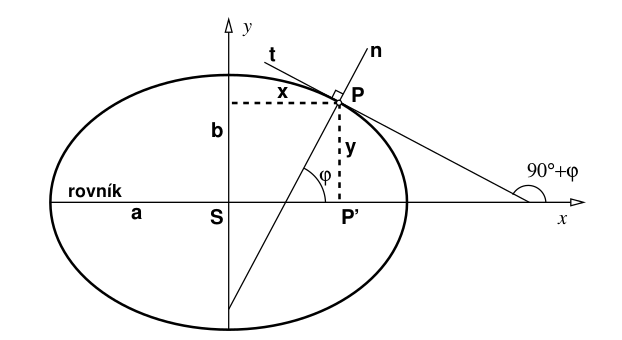
\includegraphics[width=0.60\textwidth]{FIG/CimbalnikObr1-14}
\caption{$\varphi$ $\rightarrow$ $\left(x, y\right)$. Obrázek je převzat z \cite{Cimbalnik1997}.}
\label{fig:cim114}
\end{center}
\end{figure}

Na obr. \ref{fig:cim114} svírá normála \textit{n} v bode \textbf{P} k elipse s 
velkou poloosou \textit{a} (s osou \textit{x} ) úhel $\varphi$ (geodetická šířka 
bodu \textbf{P} ). Odpovdidající tečna \textit{t} svíra s kladným směrem osy 
\textit{x} úhel $90^{\circ} + \varphi$ a její směrnice \textit{k} je dána vzorcem

\begin{equation}
k = \dfrac{dy}{dx} = \tan{\left(90^{\circ} + \varphi\right)} = -\cot{\left(\varphi\right)}.
\end{equation}
Diferencovaním rovnice meridiánové elipsy

\begin{equation}
\dfrac{x^{2}}{a^{2}} + \dfrac{y^{2}}{b^{2}} -1 = 0
\end{equation}
dostaneme

\begin{equation}
\dfrac{2xdx}{a^{2}} + \dfrac{2ydy}{b^{2}} = 0
\end{equation}
a odtud

\begin{equation}
\dfrac{dy}{dx} = - \dfrac{b^{2}x}{a^{2}y}.
\end{equation}
Z předchádzejícich rovníc vyplývá

\begin{equation}
\cot{\left(\varphi\right)} = \dfrac{b^{2}x}{a^{2}y} = \dfrac{\cos{\left(\varphi\right)}}{\sin{\left(\varphi\right)}}.
\end{equation}
Po umocnění a úpravě

\begin{equation}
b^{4}x^{2}\sin^{2}{\left(\varphi\right)} - a^{4}y^{2}\cos^{2}{\left(\varphi\right)} = 0
\end{equation}
a dále víme, že

\begin{equation}
b^{2}x^{2} + a^{2}y^{2} - a^{2}b^{2} = 0.
\end{equation}
Řešením těchto dvou (pro $x^{2}, y^{2}$ lineárních) rovníc dostaneme

\begin{equation}
x =\dfrac{a^{2}\cos{\left(\varphi\right)}}{\sqrt{a^{2}\cos^{2}{\left(\varphi\right)} + b^{2}\sin^{2}{\left(\varphi\right)}}}
\end{equation}
a
\begin{equation}
y =\dfrac{b^{2}\sin{\left(\varphi\right)}}{\sqrt{a^{2}\cos^{2}{\left(\varphi\right)} + b^{2}\sin^{2}{\left(\varphi\right)}}}.
\end{equation}
Do jmenovatelu dosaďme $b^{2} = a^{2}\left(1-e^{2}\right)$, potom po úpravě dostaneme

\begin{equation}
x =\dfrac{a\cos{\left(\varphi\right)}}{\sqrt{1-e^{2}\sin^{2}{\left(\varphi\right)}}} = \dfrac{a\cos{\left(\varphi\right)}}{W}
\label{rov:cimbX}
\end{equation}
a
\begin{equation}
y =\dfrac{a\left(1-e^{2}\right)\sin{\left(\varphi\right)}}{\sqrt{1-e^{2}\sin^{2}{\left(\varphi\right)}}} = \dfrac{a\left(1-e^{2}\right)\sin{\left(\varphi\right)}}{W},
\label{rov:cimbY}
\end{equation}
kde 
$W = \sqrt{1-e^{2}\sin^{2}{\left(\varphi\right)}}$ je první geodetická funkce.

Polohu bodu \textit{P} na rotačním elipsoidu vyjadříme v pravouhlé soustavě souřadnic. Její počátek je v středu elipsoidu \textit{S}, osa \textit{Z} v ose rotace, osa \textit{X} v průsečníku roviny rovníku s rovinou nultého poledníku, osa \textit{Y} v rovnině rovníku kolmá na osu \textit{X} - tak jak je to znázorneno na obrázku \ref{fig:cim116}.

\begin{figure}[ht!]
\begin{center}

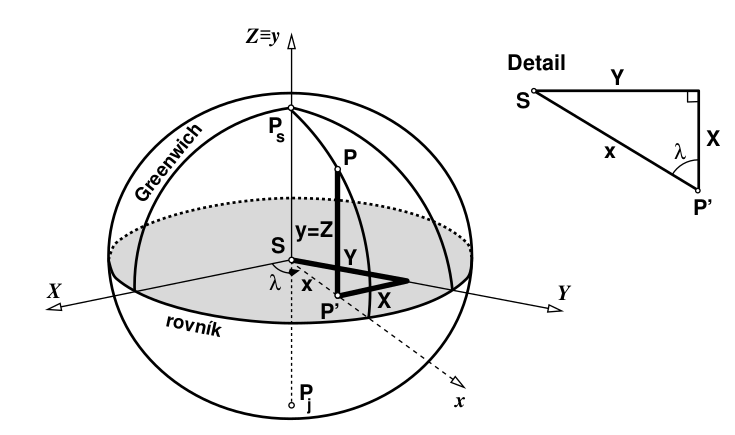
\includegraphics[width=0.60\textwidth]{FIG/CimbalnikObr1-16}
\caption{Prostorové pravouhlé souřadnice. Obrázek je převzat z \cite{Cimbalnik1997}.}
\label{fig:cim116}
\end{center}
\end{figure}

Bodem $P\left(\varphi, \lambda\right)$ prochází poledník $P_{s}-P-P_{j}-P_{s}$ o geodetické délke $\varphi$. V rovině tohto poledníku má bod \textit{P} pravouhlé souřadnice \textit{x, y}, odvozené vzorci \ref{rov:cimbX}, \ref{rov:cimbY}.

Podle obrázka \ref{fig:cim116} napíšeme pro souřadnice \textit{X, Y, Z} bodu \textit{P} vzorce

\begin{eqnarray}
X &=& x\cos{\left(\lambda\right)} \\
Y &=& x\sin{\left(\lambda\right)} \\
Z &=& y. 
\end{eqnarray}
Dosadíme-li do předchozích vzorců za x a y rovnice \ref{rov:cimbX} a \ref{rov:cimbY}, dostaneme

\begin{eqnarray}
X &=& \dfrac{a}{W}\cos{\left(\varphi\right)}\cos{\left(\lambda\right)} \\
Y &=& \dfrac{a}{W}\cos{\left(\varphi\right)}\sin{\left(\lambda\right)} \\
Z &=& \dfrac{a}{W}\left(1-e^{2}\right)\sin{\left(\varphi\right)}.
\end{eqnarray}
Uvážime-li vzorec pro příčný poloměr křivosti 
\begin{equation}
N = \dfrac{a}{W},
\end{equation}
potom geocentrické pravouhlé souřadnice bodu \textit{P} budou mít vzorce

\begin{equation}
\begin{bmatrix}
X\\
Y\\
Z
\end{bmatrix} = 
\begin{bmatrix}
N\cos{\left(\varphi\right)}\cos{\left(\lambda\right)}\\
N\cos{\left(\varphi\right)}\sin{\left(\lambda\right)}\\
N\left(1-e^{2}\right)\sin{\left(\varphi\right)}
\end{bmatrix}.
\end{equation}

V případe, že bod \textit{P} leží ve směru normály k elipsoidu ve výšce \textit{H} nad elipsoidem, pak předchozí rovnice budou
\begin{equation}
\begin{bmatrix}
X\\
Y\\
Z
\end{bmatrix} = 
\begin{bmatrix}
\left(N+H\right)\cos{\left(\varphi\right)}\cos{\left(\lambda\right)}\\
\left(N+H\right)\cos{\left(\varphi\right)}\sin{\left(\lambda\right)}\\
\left(N\left[1-e^{2}\right]+H\right)\sin{\left(\varphi\right)}
\end{bmatrix}.
\label{rov:geodEcef}
\end{equation}

Předpokládejme, že kovarianční matice souřadníc $\varphi, \lambda\ \text{a}\ H$, $\Sigma_{GEOD}$ je známá. Pro odhad kovarianční matice prostorových pravouhlých souřadníc \textit{X, Y, Z}, $\Sigma_{ECEF}$ budeme postupovať podle článku Transformace kovariančních matíc. Z článku víme, že úlohou je vyjádřít Jakobiho matici $\textbf{J}$. Derivovaním modelu rovníc \textit{X, Y, Z} z poslední rovníce podle veličín $\varphi, \lambda\ \text{a}\ H$, postupně dostaneme:

\begin{equation}
\mathbf{J} = 
\begin{bmatrix}
\dfrac{\partial X}{\partial \varphi} & \dfrac{\partial X}{\partial \lambda} & \dfrac{\partial X}{\partial H} \\
\dfrac{\partial Y}{\partial \varphi} & \dfrac{\partial Y}{\partial \lambda} & \dfrac{\partial Y}{\partial H} \\
\dfrac{\partial Z}{\partial \varphi} & \dfrac{\partial Z}{\partial \lambda} & \dfrac{\partial Z}{\partial H}.
\end{bmatrix}
\end{equation}
Pro jednotlivé zložky platí:

\begin{equation}
\dfrac{\partial X}{\partial \varphi} = \cos{\left(\lambda\right)}\left(\dfrac{\partial N}{\partial \varphi}\cos{\left(\varphi\right)}-\sin{\left(\varphi\right)}\left(N + H\right)\right),
\end{equation}

\begin{equation}
\dfrac{\partial X}{\partial \lambda} = -\left(N+H\right)\cos{\left(\varphi\right)}\sin{\left(\lambda\right)},
\end{equation}

\begin{equation}
\dfrac{\partial X}{\partial H} = \cos{\left(\varphi\right)}\cos{\left(\lambda\right)},
\end{equation}

%sin(lon) * (dNdLat * cos(lat) - vertRad * sin(lat) - hgt * sin(lat));
\begin{equation}
\dfrac{\partial Y}{\partial \varphi} = \sin{\left(\lambda\right)}\left(\dfrac{\partial N}{\partial \varphi} \cos{\left(\varphi\right)} - \sin{\left(\varphi\right)}\left(N + H\right)\right),
\end{equation}

\begin{equation}
\dfrac{\partial Y}{\partial \lambda} = \left(N+H\right)\cos{\left(\varphi \right)}\cos{\left(\lambda \right)},
\end{equation}

\begin{equation}
\dfrac{\partial Y}{\partial H} = \cos{\left(\varphi \right)}\sin{\left(\lambda \right)},
\end{equation}

\begin{equation}
\dfrac{\partial Z}{\partial \varphi} = \dfrac{b^{2}}{a^{2}}\left(\sin{\left( \varphi\right)} \dfrac{\partial N}{\partial \varphi} + \cos{\left( \varphi \right)} N \right) + H\cos{\left( \varphi \right)},
\end{equation}

\begin{equation}
\dfrac{\partial Z}{\partial \lambda} = 0,
\end{equation}

\begin{equation}
\dfrac{\partial Z}{\partial H} = \sin{\left( \varphi \right)},
\end{equation}
kde
\begin{equation}
\dfrac{\partial N}{\partial \varphi} = \dfrac{a e^{2} \sin{\left(\varphi\right)}\cos{\left(\varphi\right)}}{\left(1-e^{2}\sin^{2}{\left(\varphi\right)}\right)^{3/2}}
\end{equation}
a veličiny \textit{a, e, N} jsou hlavní poloos meridiánové elipsy, její první excentricita a příčný poloměr křivosti.

Kovarianční matice souřadníc prostorového pravouhlého souřadnicového systému ECEF je s přihlédnutím k právě definované Jakobiho matici
\begin{equation}
\mathbf{\Sigma}_{ECEF} = \mathbf{J}\mathbf{\Sigma}_{GEOD}\mathbf{J}^{T}.
\end{equation}

\subsubsection{Příklad transformace z GEOD $\rightarrow$ ECEF}

Ukážme si příklad transformace z geodetických souřadníc do prostorových pravouhlých souřadníc.

Bod \textit{P} ležíci na elipsoidu má geodetické spuřadnice:
\begin{itemize}
\item $\varphi = 48.8562^{\circ}$
\item $\lambda = 2.3508^{\circ}$
\item $h = 0.0674 m.$
\end{itemize}
Po aplikovaní rovnice \ref{rov:geodEcef} (uvažujeme rotační elipsoid WGS-84 tak jak je definován v \ref{appRefEllConstWGS84}), prostorové geocentrické souřadnice bodu \textit{P} jsou:
\begin{itemize}
\item $X = 4200952.53 m$
\item $Y = 172458.50 m$
\item $Z = 4780052.13 m.$
\end{itemize}

Pseudokód Matlab funkce geod2ecef(), která je implmentováná v package +Geo Package je obsahem přílohy \ref{appGeod2Ecef}.


\subsection{ECEF $\rightarrow$ GEOD}

Existuje celá řada metod, které se zaměřují na inversní transformaci souřadnic z pravoúhlého prostorového systému souřadnic na systém geodetických zeměpisných souřadnic. Práce se speciálně zaměřují na převod geodetické šířky $\varphi$ a to hlavně z důvodu přesnosti jejího odhadu (víme, že z důvodu zploštění referenčního tělesa, v našem případě elipsoidu, geodetická šířka není definována na spojnici středu elipsoidu a bodu \textit{P} na povrchu elipsoidu a proto nastávají problémy řešení rovnice pro odhad geodetické šířky ze vstupních parametrů, které jsou pravoúhlé geocentrické souřadnice) nebo z důvodu výpočetního (geodetická šířka se počítá buď iterativními metodami nebo neiterativními). Z odborných článků, které se věnují tomuto problému bychom mohli citovat například \cite{Bowring1976}, \cite{Borkowski1989} nebo z aktuálních prací \cite{Fukushima2006} či \cite{Vermeille2011} (implementován v + Geo package). Autoři, v práci \cite{Fok2003} se věnovali vzájemnému srovnání vybraných (do toho roku známých) algoritmů.

Jeden ze základních algoritmů (bez ověření přesnosti či výpočetní rychlosti) na odhad geodetických souřadnic $ \left(\varphi, \lambda, h \right)$ počítaných z pravoúhlých kartézskych souřadnic X, Y, Z je tento \cite{Grewal2001}:


\begin{equation}
\lambda = \tan^{-1}{\left(\dfrac{Y}{X}\right)},
\end{equation} 

\begin{equation}
\varphi = \tan^{-1}{\left(\dfrac{Z+\dfrac{e^{2}a^{2}\sin^{3}{\left(\zeta\right)}}{b}}{\xi-e^{2}a\cos{\left(\zeta\right)}}\right)},
\end{equation} 

a

\begin{equation}
h = \dfrac{\xi}{\cos{\left(\varphi\right)}} - N,
\end{equation}
kde

\begin{equation}
\zeta = \tan^{-1}{\left(\dfrac{aZ}{b\xi}\right)}
\end{equation}

\begin{equation}
\xi = \sqrt{X^{2} + Y^{2}}, 
\end{equation}
a \textit{N} je příčný poloměr křivosti, \textit{a} je hlavní poloosa meridiánové elipsy, \textit{b} je vedlejší poloosa meridiánovej elipsy a \textit{e} je její excentricita.

Odhad kovarianční matice geodetických souřadníc bodu v geodetickém souřadnicovém systému nebude záviset na komplikovaných iteračních postupech spojených s odhadem zeměpisné šiřky. S výhodou využijeme výsledných rovníc popsaných v části textu, kde se věnujeme transformaci geodetických souřadníc bodu do systému prostorových pravouhlých souřadníc, respektíve transformační Jacobiho matice, kterou jsme z těchto rovníc odvodili. Inverze takto odvozené Jacobiho matice nám v této časti poslouži k odhadu kovarianční matice výsledných geodetických souřadníc. Proto pro kovariační matici geodetických souřadníc transformované ze soustavy prostorových souřadníc bude

\begin{equation}
\mathbf{\Sigma}_{GEOD} = \mathbf{J}^{-1}\mathbf{\Sigma}_{ECEF}\left(\mathbf{J}^{-1}\right)^{T}.
\end{equation}

\subsubsection{Příklad transformace z ECEF $\rightarrow$ GEOD}

Příklad transformace z prostorových pravouhlých souřadníc do systému geodetických souřadníc.

Bod \textit{P} ležíci na elipsoidu má tentokrát prostorové  spuřadnice:
\begin{itemize}
\item $X = 4200952.53 m$
\item $Y = 172458.50 m$
\item $Z = 4780052.13 m.$
\end{itemize}

Po aplikovaní algoritmu například \cite{Vermeille2011} (uvažujeme rotační elipsoid WGS-84 tak jak je definován v \ref{appRefEllConstWGS84}), pak prostorové geocentrické souřadnice bodu \textit{P} jsou:
\begin{itemize}
\item $\varphi = 48.8562^{\circ}$
\item $\lambda = 2.3508^{\circ}$
\item $h = 0.0674 m.$
\end{itemize}

Pseudokód Matlab funkce ecef2geod(), která je implmentováná v package +Geo Package je obsahem přílohy \ref{appEcef2Geod}.

\subsection{ENU $\rightarrow$ AES}

Algoritmus určený na odhad polárnych súradníc (Az - azimut, El - elevačný uhol a Sr - šikmá spojnica medzi lokálnym počiatkom a cieľom) počítaných s lokálnych pravouhlých súradníc napríklad súradného systému ENU je tento:

\begin{eqnarray}
\tan\left(Az\right) &=& \dfrac{E}{N}, \\
\tan\left(El\right) &=& \dfrac{U}{\sqrt{E^{2} + N^{2}}}, \\
Sr &=& \sqrt{E^2 + N^2 + U^2}.
\end{eqnarray}

\subsubsection{Příklad transformace z ENU $\rightarrow$ AES}

Příklad transformace z lokálnich pravouhlých souřadníc do systému polárních souřadníc.

Bod \textit{P}, například cíl, kterého poloha je charakterizováná v souřadnicovém systému ENU má prostorové  spuřadnice:
\begin{itemize}
\item $E = 8.4504 m$
\item $N = 12.4737 m$
\item $U = 1.1046 m.$
\end{itemize}

Polárne souřadnice tohto cíle jsou:
\begin{itemize}
\item $Az = 34.1160^{\circ}$
\item $El = 4.1931^{\circ}$
\item $Sr = 15.1070 m.$
\end{itemize}

\subsection{AES $\rightarrow$ ENU}

Spätný algoritmus určený na odhad lokálnych pravouhlých súradníc (E - East, N - North, U - Up) počítaných z plárnych súradníc AES (Az - azimut, El - elevačný uhol a Sr - šikmá spojnica medzi lokálnym počiatkom a cieľom) je tento:

\begin{eqnarray}
E &=& Sr\cdot \cos{\left(El\right)}\cdot \sin{\left(Az\right)}, \\
N &=& Sr\cdot \cos{\left(El\right)}\cdot \cos{\left(Az\right)}, \\
U &=& Sr\cdot \sin{\left(El\right)} .
\end{eqnarray}

\subsubsection{Příklad transformace z AES $\rightarrow$ ENU}

Bod \textit{P}, je definovnám pomocu polárních souřadníc.
\begin{itemize}
\item $Az = 34.1160^{\circ}$
\item $El = 4.1931^{\circ}$
\item $Sr = 15.1070 m.$
\end{itemize}

Lokálni pravouhlé souřadnice tohto cíle jsou:
\begin{itemize}
\item $E = 8.4504 m$
\item $N = 12.4737 m$
\item $U = 1.1046 m.$
\end{itemize}



\section{Vybrané kartografické zobrazení}

Z hlediska zkreslení zobrazení rozlišujeme na:
\begin{enumerate}
\item konformní - stejnouhlá,
\item ekvidistantní - stejnodelná,
\item ekvivalentní - stejnoplochá,
\item kompenzační - vyrovnávací.
\end{enumerate}

Z pohledu k třídění zobrazovací plochy, pomocí které si můžeme představit vznik obrazu referernční lochy rozlišujeme:
\begin{enumerate}
\item zobrazení na kulovou plochu,
\item jednoduchá zobrazení (kuželová, válcová, azimutální),
\item nepravá zobrazení (pseudokonická, pseudocylindrická, pseudoazimutální),
\item polykónická,
\item polyederická, 
\item obecná.
\end{enumerate}
My popíšeme jenom vybrané jednoduchá zobrazení a to konrkétně válcová (UTM) a azitmální (stereografická projekce).

\subsection{Definice a některé vlastnosti vybraných kartografického zobrazení}

Kartografickým zobrazením je podle \cite{Buchar2002} vzájemné přiřazení polohy bodů na dvou různých referenčních plochách. V některých případech, kdy je možno vztah realizovat geometrickou cestou (promítaním), podle \cite{Buchar2002} budeme takové zobrazení nazývat projekcí neboli prospektivním zobrazením.

Zobrazení je jednoznačne matematicky definováno vtahem mezi souřadnicemi bodů na oboureferenčních plochách, kterému říkame zobrazovací rovnice. Například zobrazení elipsoidu do roviny budou zobrazovací rovnice v explicitním tvaru

\begin{equation}
X = f\left(\varphi, \lambda\right),
\end{equation}


\begin{equation}
Y = g\left(\varphi, \lambda\right),
\end{equation}
kde funkce \textit{f, g} v určitém místě považujeme za spojité, obecně na sobě mezávislé, diferencovatelné apod. Výjimky představují singulární body (např. póly), kde uvedená vlastnost není obecně splněna.

\subsubsection{Poznámky k jednoduchým zobrazením}
Pro naše účely nás budou zajímat jenom jednoduchá zobrazení. Jednoduchá zobrazní jsou taková zobrazení, pro něž je možno zapsat zobrazovací rovnice, podle nichž každá  z rovinných souřadníc (polárních nebo pravoúhlých) a výrazy pro zkreslení (zýávislé proměnné) se dají vyjádřit funkcemi pouze jedné souřadnice (nezávsilé proměnné) na referenční ploše. Důsledkem takové jednoduché volby je pak i jednoduchý obraz poledníků a rovnobežek, které jsou pak na mapě znázorněny jako svazek přímek čo osnova rovnoběřných přímek (u poledníku) a soustava rovnoběžných kružnic či osnova rovnoběžných přímek (u rovnoběžek). Jednoduchá zobrazení jsou ortogonální (viz \cite{Buchar2002}, str. 51).

\subsection{Poznámky k valcovým zobrazením}
Válcová zobrazení v normálni poloze mají tyto vlastnosti \cite{Buchar2002}:
\begin{enumerate}
\item rovník a rovnoběžky se zobrazují jako osnova rovnoběžných přímek,
\item obrazy poledníků tvoří osnovu přímek vzájemně stejně odlehlých rovnoběžných a kolmých na obrazy rovnoběžek,
\item obraz základního poledníku volíme jako osu Y, 
\item zobrazovací rovnica pro Y je veličina Y funkcí pouze $\left(\varphi\right)$.
\item do obrazou rovníku vkládame osu X (u souřadnícových systému používaných v geodézii je orientace opačná),
\item zobrazovací rovnica pro X je X lineární funkcí zeměpisné délky $\left(\lambda\right)$.
\end{enumerate}

Zkreslení v poledníku a rovnoběžce jsou:
\begin{equation}
m_{p} = \dfrac{dY}{M d\varphi}
\label{rov:zkresValPol}
\end{equation}

\begin{equation}
m_{r} = \dfrac{dX}{N \cos{\left(\varphi\right)d\lambda}} = \dfrac{a}{N\cos{\left(\varphi\right)}},
\label{rov:zkresValRov}
\end{equation}
kde \textit{M, N} jsou meridiánový a příčný poloměr křivosti, \textit{a} je hlavní poloosa meridiánové elipsy a $\varphi$ je zeměpisná šířka.

Protože poledník a rovnoběžka tvoří u válcových zobrazení hlavní paprsky, je pro konformitu jedinou a postačující podmínkou

$$m_{p} = m_{r},$$ 
a pri referenční ploše elipsoidické a nezkresleném rovníku bude pro dosazení \ref{rov:zkresValPol} a \ref{rov:zkresValRov}, platit:
\begin{equation}
\dfrac{dY}{M d\varphi} = \dfrac{a}{N\cos{\left(\varphi\right)}}.
\end{equation}
Po separaci proměnných dostaneme
\begin{equation}
dY = a\dfrac{M}{N\cos{\left(\varphi\right)}}d\varphi,
\label{rov:dY}
\end{equation}
kde na pravé straně rovnice se vyskytuje výraz pro tzv. izometrickou šířku.

Izometrická šířka \textit{q}, která je funkcí zeměpisné šířky $\varphi$, je definováná:
\begin{equation}
q = \int_{0}^{\varphi}\dfrac{M}{N\cos{\left(\varphi\right)}}d\varphi
\end{equation}
a po dosazení za \textit{M} a \textit{N} dostaneme
\begin{eqnarray}
q &=& \int_{0}^{\varphi} \dfrac{\left(1-e^{2}\right)}{\left(1-e^{2}\sin^{2}{\left(\varphi\right)}\right)\cos{\left(\varphi\right)}}d\varphi \\ \nonumber
  &=&\int_{0}^{\varphi}\dfrac{\left(1-e^{2}\sin^{2}{\left(\varphi\right)}-e^{2}\cos^{2}{\left(\varphi\right)}\right)d\varphi}{\left(1-e^{2}\sin^{2}{\left(\varphi\right)}\right)\cos{\left(\varphi\right)}} \\ \nonumber
  &=& \int_{0}^{\varphi}\dfrac{d\varphi}{\cos{\left(\varphi\right)}} - \int_{0}^{\varphi}\dfrac{e\cos{\left(\varphi\right)}d\varphi}{1-e^{2}\sin^{2}{\left(\varphi\right)}} \\ \nonumber
  &=& \ln\tan{\left(\dfrac{\varphi}{2} + \dfrac{\pi}{4}\right)} - e\int_{0}^{\varphi}\dfrac{d\left(e\sin{\left(\varphi\right)}\right)}{1-e^{2}\sin^{2}{\left(\varphi\right)}},
\end{eqnarray}
a po proložení $x = e\sin{\left(\varphi\right)}$ v posledním integrálu, z nehož plyne, že 
\begin{equation}
\int \dfrac{dx}{1-x^{2}} = \dfrac{1}{2}\ln{\left(\dfrac{1+x}{1-x}\right)} = \dfrac{1}{2}\ln{\left(\dfrac{1+e\sin{\left(\varphi\right)}}{1-e\sin{\left(\varphi\right)}}\right)}
\end{equation}
a pro izometrickou šířku pak platí
\begin{equation}
q = \ln{\left[\tan{\left(\dfrac{\varphi}{2}+\dfrac{\pi}{4}\right)}\left( \dfrac{1-e\sin{\left(\varphi\right)}}{1+e\sin{\left(\varphi\right)}} \right)^{\dfrac{e}{2}}\right]}.
\label{rov:izometricka}
\end{equation}
Po dosazení \ref{rov:izometricka} do \ref{rov:dY} dostaneme \cite{Buchar2002}, \cite{Snyder1987}:
\begin{equation}
Y = a\ln{\left[\tan{\left(\dfrac{\varphi}{2}+\dfrac{\pi}{4}\right)}\left( \dfrac{1-e\sin{\left(\varphi\right)}}{1+e\sin{\left(\varphi\right)}} \right)^{\dfrac{e}{2}}\right]}.
\label{rov:utmY}
\end{equation}
Protože \textit{X} je lineární funkce zeměpisné délky, pro vyjdřední souřadnice \textit{X} platí:
\begin{equation}
X = a\left(\lambda-\lambda_{0}\right).
\end{equation}

Inversní vzorec pro veličinu $\varphi$ v případě spětné transformace vyžaduje počítaní přes iterační proces a základní rovnice je definováná ve tvaru \cite{Snyder1987}

\begin{equation}
\varphi = \dfrac{\pi}{2} - 2 \tan^{-1}{\left\lbrace t \left[ \dfrac{1-e\sin{\left(\varphi\right)}}{1+e\sin{\left(\varphi\right)}} \right]^{\dfrac{e}{2}} \right\rbrace}, 
\end{equation}
kde
$$t = e^{\dfrac{-Y}{a}}$$
a iterační proces začína výpočtem
$$\varphi = \dfrac{\pi}{2}-2\tan^{-1}{\left(t\right)}$$
a pokračuje pokud není dosažení zvolená konvergenční hranice.

Inversní zeměpisná délka se vypočte podle rovnice:
\begin{equation}
\lambda = \dfrac{X}{a} + \lambda_{0}.
\end{equation} 

\subsubsection*{Konformní transversální válcové zobrazení}

Konformní transversální válcové zobrazení nazývané také Gaussovo (pro elipsoidickou referenční plochu) nebo transversální Mercatorovo, je specifické tím, že válec  se dotýka referenční koule (elipsoidu) podél základního poledníku, procházejíciho středem území. Kartografické poledníky a rovnoběžky se pak zobrazují jako zeměpisné polidníky a rovnoběžky v normálni poloze. 

Uplatnění našlo také konformní válcové zobrazení v obecné poloze (v literatuře Oblique Mercator Projection). Délkově zachovává zvolený kartografický rovník.

\subsubsection*{Universální transversální zobrazení v poledníkových pásech, zobrazení systému UTM}

V zobrazeních, v kterých má být užito v poloze jiné než normální, zobrazuje se najdřív elipsoid na kouli a pak terpve s koule na zobrazovací plochu, \cite{Buchar2002}. V případě Gauss (Gauss-Kr\"{u}gerova) zobrazení, elipsoid je zobrazován přímo do roviny, tedy bez zprostředkujíci koule a to tak, že meridiální pruhy stejné šířky se zobrazují samostatně. Určující podínkou je konformita a nezkreslený základní (střední) poledník pásu. 

\subsection{GEOD$\rightarrow$ UTM}

V knize \cite{Buchar2002} se uvádí podrobné odvození zobrazovacích rovníc. Z pohledu programatorského je možná výhodnějnší popsat algoritmus, který se nachádzí v knize \cite{Snyder1987} (vzorce platí pro elipsoid).

\begin{equation}
x = k_{0}N\left[A + \left(1-T+C\right)\dfrac{A}{6} + \left(5-18T+T^{2}+72C-58e^{'2}\right)\dfrac{A^{5}}{120}\right]
\end{equation}	

\begin{equation}
y = k_{0}\left\lbrace B - B_{0} + N \tan{\left(\varphi\right)\left[\dfrac{A^{2}}{2} + \left(5-T+9C+4C^{2}\right)\dfrac{A^{4}}{24}+\left(61-58T+T^{2}+600C-330e^{'2}\right)\dfrac{A^{6}}{720}\right]}\right\rbrace
\end{equation}

\begin{equation}
k = k_{0}\left[1+\left(1+C\right)\dfrac{A^{2}}{2}+\left(5-4T+42C+13C^{2}-28e^{'2}\right)\dfrac{A^{4}}{24} + \left(61-148T+16T^{2}\right)\dfrac{A^{6}}{720}\right],
\end{equation}
kde
\begin{itemize}
\item $k_{0}$ je multipliační konstanta $k_{0} = 0.9996$,
\item $e^{'2}$ je druhá excentricita rotačního eliposidu definováná také pomocí $e^{'2} = e^{2}/\left(1-e^{2}\right)$,
\item $N$ je příčný poloměr křivosti rotačního elipsoidu, 
\item $T = \tan^{2}{\left(\varphi\right)}$,
\item $C = e^{'2}\cos^{2}{\left(\varphi\right)}$,
\item $A = \left(\lambda-\lambda_{0}\right)\cos{\left(\varphi\right)}$ předpokladajíc, že $\lambda\ \text{a}\ \lambda_{0}$ jsou v radiánech,
\item $B$ je délka oblouku meridiánu od rovníku po $\varphi$. $B_{0} = B$ zpočtěná pro $\varphi_{0}$ a platí
\begin{eqnarray}\label{rov:B}
B = & a & \left(1 - \dfrac{e^{2}}{4} - \dfrac{3e^{4}}{64} - \dfrac{5e^{6}}{256} - \cdots \right)\varphi \\ \nonumber
    & -a & \left(\dfrac{3e^{2}}{8} + \dfrac{3e^{4}}{32} + \dfrac{45e^{6}}{1024} - \cdots\right)\sin{\left(2\varphi\right)}\\ \nonumber
    & +a & \left(\dfrac{15e^{4}}{256} + \dfrac{45e^{6}}{1024} + \cdots\right)\sin{\left(4\varphi\right)}\\ \nonumber
    & -a & \left(\dfrac{35e^{6}}{3072} + \cdots\right)\sin{\left(6\varphi\right)}\\ \nonumber
\end{eqnarray}
\item $\varphi$ je zeměpisná délka v radiánech.
\end{itemize}

Pokud $\varphi \pm \pi/2$, pak $x=0$, $y = k_{0}\left(B-B_{0}\right)$ a $k=k_{0}$.

Jednotlivé osi souřadníc jsou dané takto: Yová osa leži v obraze základnáho poledníku $\lambda_{0}$ a y roste směrem na sever. Xová osa je kolmá na Y a x roste směrem na východ. 

\subsection{UTM $\rightarrow$ GEOD}

Pro inversní vzroce podle \cite{Snyder1987}  platí:
\begin{eqnarray}
\varphi = \varphi_{1} &-& G\left[\dfrac{D^{2}}{2}-\left(5+3T_{1}+10C_{1}-4C_{1}^{2}-9e^{'2}\right)\dfrac{D^{4}}{24}\right] \\ \nonumber
                      &-& G\left[\left(61+90T_{1}+298C_{1}+45T_{1}^{2}-252e^{'2}-3C_{1}^{2}\right)\dfrac{D^{6}}{720}\right], 
                      \label{rov:invPhi}
\end{eqnarray}

\begin{eqnarray}
\lambda = \lambda_{0} + \dfrac{D-\left(1+2T_{1}+C_{1}\right)\dfrac{D^{3}}{6} + \left(5-2C_{1}+28T_{1}-3C_{1}^{2}+8e^{'2} + 24T_{1}^{2}\right)\dfrac{D^{5}}{120}}{\cos{\left(\varphi_{1}\right)}},
\label{rov:invLam}
\end{eqnarray}
kde

\begin{itemize}
\item $G = \left(\dfrac{N_{1}\tan{\left(\varphi_{1}\right)}}{R_{1}}\right)$
\item $\varphi_{1}$ je zeměpisná šířka charakteristická pro centrální meridián a která ma stejnou \textit{y} souřadnici jako bod, kterého polární sořadnice jsou $\left(\varphi, \lambda\right)$ 
\begin{eqnarray} \nonumber
\varphi_{1} = \mu &+& \left( \dfrac{3e_{1}}{2} - \dfrac{27e_{1}^{3}}{32} + \cdots \right)\sin{2\mu} \\ \nonumber
                  &+& \left( \dfrac{21e_{1}}{16} - \dfrac{55e_{1}^{4}}{32} + \cdots \right)\sin{4\mu} \\ \nonumber
                  &+& \left( \dfrac{151e_{1}^{3}}{96} + \cdots \right)\sin{6\mu} \\ \nonumber
                  &+& \left( \dfrac{1097e_{1}^{4}}{512} - \cdots \right)\sin{8\mu} \nonumber
\end{eqnarray}
\item $
e_{1} = \dfrac{1 - \sqrt{1-e^{2}}}{1 + \sqrt{1-e^{2}}}
$
\item $\mu = \dfrac{B}{a\left(1-\dfrac{e^{2}}{4} - \dfrac{3e^{4}}{64} - \dfrac{5e^{6}}{256} - \cdots\right)} 
$
\item $B_{0}$ je spočtená pomocí rovnice \ref{rov:B} pro vstupní $\varphi_{0}$,
\item $B = B_{0} + \dfrac{y}{k_{0}}$,
\item $e^{'2} = \dfrac{e^{2}}{\left(1-e^{2}\right)}$,
\item $C_{1} = e^{'2}\cos^{2}{\left(\varphi_{1}\right)}$,
\item $T_{1} = \tan^{2}{\left(\varphi_{1}\right)}$,
\item $N_{1} = \dfrac{a}{\sqrt{\left(1-e^{2}\sin^{2}{\left(\varphi_{1}\right)}\right)}}$,
\item $R_{1} = \dfrac{a\left(1-e^{2}\right)}{\left(1-e^{2}\sin^{2}{\left(\varphi_{1}\right)}\right)^{3/2}}$,
\item $D = \dfrac{x}{N_{1}k_{0}}$.
\end{itemize}

\subsubsection*{Meridiánová konvergence}
Meridiánová konvergence je podle \cite{webVUGTK} úhel určitém bodu referenční plochy mezi tečnami k místnímu poledníku a ke křivce rovnoběžné se základním poledníkem; může být elipsoidická meridiánová konvergence, sférická meridiánová konvergence a rovinná meridiánová konvergence.

V knize \cite{Buchar2002}, vzorec pro výpočet meridiánové konvergence $\gamma$ je (bez odvození)
\begin{eqnarray}
\tan{\left(\gamma\right)} &=& \lambda\sin{\left(\varphi\right)} + \dfrac{\lambda^{3}}{3}\sin{\left(\varphi\right)} \cos^{2}{\left(\varphi\right)}\left(1+\tan^{2}{\left(\varphi\right)} + 3\eta^{2} + 2\eta^{4} \right)  \\ \nonumber
                         &+&\dfrac{\lambda^{5}}{15}\sin{\left(\varphi\right)} \cos^{4}{\left(\varphi\right)}\left(2+4\tan^{2}{\left(\varphi\right)} +2\tan^{4}{\left(\varphi\right)} \right) + \cdots, \nonumber
\end{eqnarray}
kde $\eta^{2} = \dfrac{e^{2}\cos^{2}{\left(\varphi\right)}}{1-e^{2}}$.

\subsubsection*{Délkové zkreslení}
Délkové zkreslení je funkcií zeměpisných souřadníc a pre jeho výpočet platí \cite{Buchar2002}:
\begin{equation}
m = 1+\dfrac{\lambda}{2}\cos^{2}{\left(\varphi\right)}.
\end{equation}
Chceme-li délkové zkreslení zpočíst z pravouhlých souřadníc, pak vzorec pre výpočet je tento:
\begin{equation}
m = 1+\dfrac{y^{2}}{2R^{2}} + \dfrac{y^{4}}{24R^{4}} + \cdots,
\end{equation}
avšak $R = \sqrt{MN}$ je funkcí zeměpisné šířky $\varphi$.



\subsection{Poznámky k azimutálním zobrazením}

Azimutální zobrazení si můžeme představit tak, že obraz referenčního tělesa vzniká již přímo v rovině \cite{Buchar2002}, str. 99. V tomto zobrazení je rovina kolmá ke spojnici kartografického pólu se sředem referenční koule (pozor na projekci z elipsoidu). Nasledujíci text se týka odvození zobrazení vývozené z referenční koule. V knize \cite{Snyder1987} se diskutuje algoritmus respektíve vzorce platné pro elipsoid.

Z azimutálniho zobrazení jsou známá některé vlastnosti, například:

\begin{itemize}
\item Obrazem poledníků je svazek přímek s vrcholem v kartografickém pólu a které svírají stejné úhly jako na kouli.
\item Základní poledník se zobrazí jako osa X.
\item Obrazem rovnoběžek jsou kružnice se středem v kartografickém pólu. Poloměr těchto rovnoběžek závisí na kartografické šiřce.
\end{itemize} 

Zobrazovací rovnice jsou:
\begin{equation}
\rho = f\left(\psi\right),
\end{equation}
kde $\psi = 90^{\circ}-\varphi$, kde v tomto případe $\varphi$ je kartografická šířka (odvozená na kouli a ne na elipsoidu).
\begin{equation}
\varepsilon = \lambda,
\end{equation}
kde $\lambda$ v tomto případe reprezentuje kartografickou délku.

Funkci \textit{f} v případě první zobrazovací rovnice definujeme na základě požadávků, nejčastěji z ekvidistance, ekvivalence či konfomity. Nás bude zajímat konformní zobrazení, protože stereografická projekce zachováva konformitu úhlů.

V azimutálním zobrazení můžeme zavést pravouhlou rovinnou soustavu, kde pravoúhlé souřadnice X, Y získame transformací polárních souřadníc na pravouhlé souřadnice. Počátek takéto souřadnicové soustavy je potom někdy vhodné pomocí aditačních konstant přesunout do libovolného místa vzhledem k středu zobrazovaného území a to tak, aby souřadnice v tomto území měly kladnou hodnotu.

K transformaci polárních souřadníc do soustavy pravouhlých souřadnic použijeme výrazy:
\begin{equation}
X = \rho \cos{\left(\varepsilon\right)},
\end{equation}

\begin{equation}
Y = \rho \sin{\left(\varepsilon\right)},
\end{equation}
resp. pro inversní případ platí:
\begin{equation}
\rho = \sqrt{X^{2} + Y^{2}},
\end{equation}
a
\begin{equation}
\varepsilon = \tan^{-1}{\left(\dfrac{Y}{X}\right)}.
\end{equation}

Jak už bylo nastíněno, nás bude zajímat konformní zobrazení. Pro  konformní azimutální zobrazení je jedninou a postačující podmínkou

\begin{equation}
\dfrac{d\rho}{Rd\psi} = \dfrac{\rho}{R\sin{\left(\psi\right)}}.
\end{equation} 
Po separaci proměnných 
\begin{equation}
\dfrac{d\rho}{\rho} = \dfrac{d\psi}{\sin{\left(\psi\right)}}
\end{equation}
a po integraci dostaneme
\begin{equation}
\ln{\left(\rho\right)} = \ln{\left(\tan{\left(\dfrac{\psi}{2}\right)}\right)} + \ln{\left(C\right)},
\end{equation}
kde \textit{C} je libovolná integrační konstanta a z poslední rovnice plyne, že
\begin{equation}
\rho = C\tan{\left(\dfrac{\psi}{2}\right)}.
\end{equation}
Pokud zavedeme podmínku, aby pro střed mapy (pro pól) platilo $m = 1$, pak (bez odvození - viz \cite{Buchar2002}), $C = 2R$, takže zobrazovací rovnice jsou
\begin{equation}
\rho = 2R\tan{\left(\dfrac{\psi}{2}\right)}
\end{equation}
a
\begin{equation}
\varepsilon = \lambda.
\end{equation}
Výraz pro zkreslení $m$ je
\begin{equation}
m = \dfrac{1}{\cos{\left(\dfrac{\psi}{2}\right)}}.
\end{equation}

Pokud chceme stanovit v pólu konkrétní délkové zkreslení různe od jedné, je možné, podobně jako v případe UTM zobrazení, zavést multiplikační konstantu, jejíž velkost udává délkové zkreslení v pólu. Platí
\begin{equation}
C = k2R.
\end{equation}

Vedle konformity má zobrazení důležitou vlastnost, že každá kružnice na referenční ploše kulové se zobrazuje opět jako kružnice. Tedy obrazy geografické sítě se skládá ze samých kružnic respektíve přímek (kružnice s nulovou křivostí).

Výraz pro délkové zrekslení je možné vyjádřit i za použití rovinných souřadníc a to v tvaru
\begin{equation}
m = 1+\dfrac{X^{2}+Y^{2}}{4R^{2}}, 
\end{equation}
kde \textit{R} je poloměr koule.

\newpage
\subsection{GEOD $\rightarrow$ STEREO}

Azimutální (geometrické) projekce vznikají promítnutím povrchu referenční koule o poloměru \textit{R} z libovolného bodu $K_{c}$ na rovinu $\pi$, kolmou ke spojnici středu promítaní $K_{c}$ se středem kolue \textit{C}. Podle předchozího obrázku, který znázorňuje osový řez rovinou promítacího paprsku bodu P, je obraz bodu $P^{'}$ určen v rovině $\pi$ polárnimi souřadnicemi $\rho, \varepsilon$.

\begin{figure}[ht!]
\begin{center}

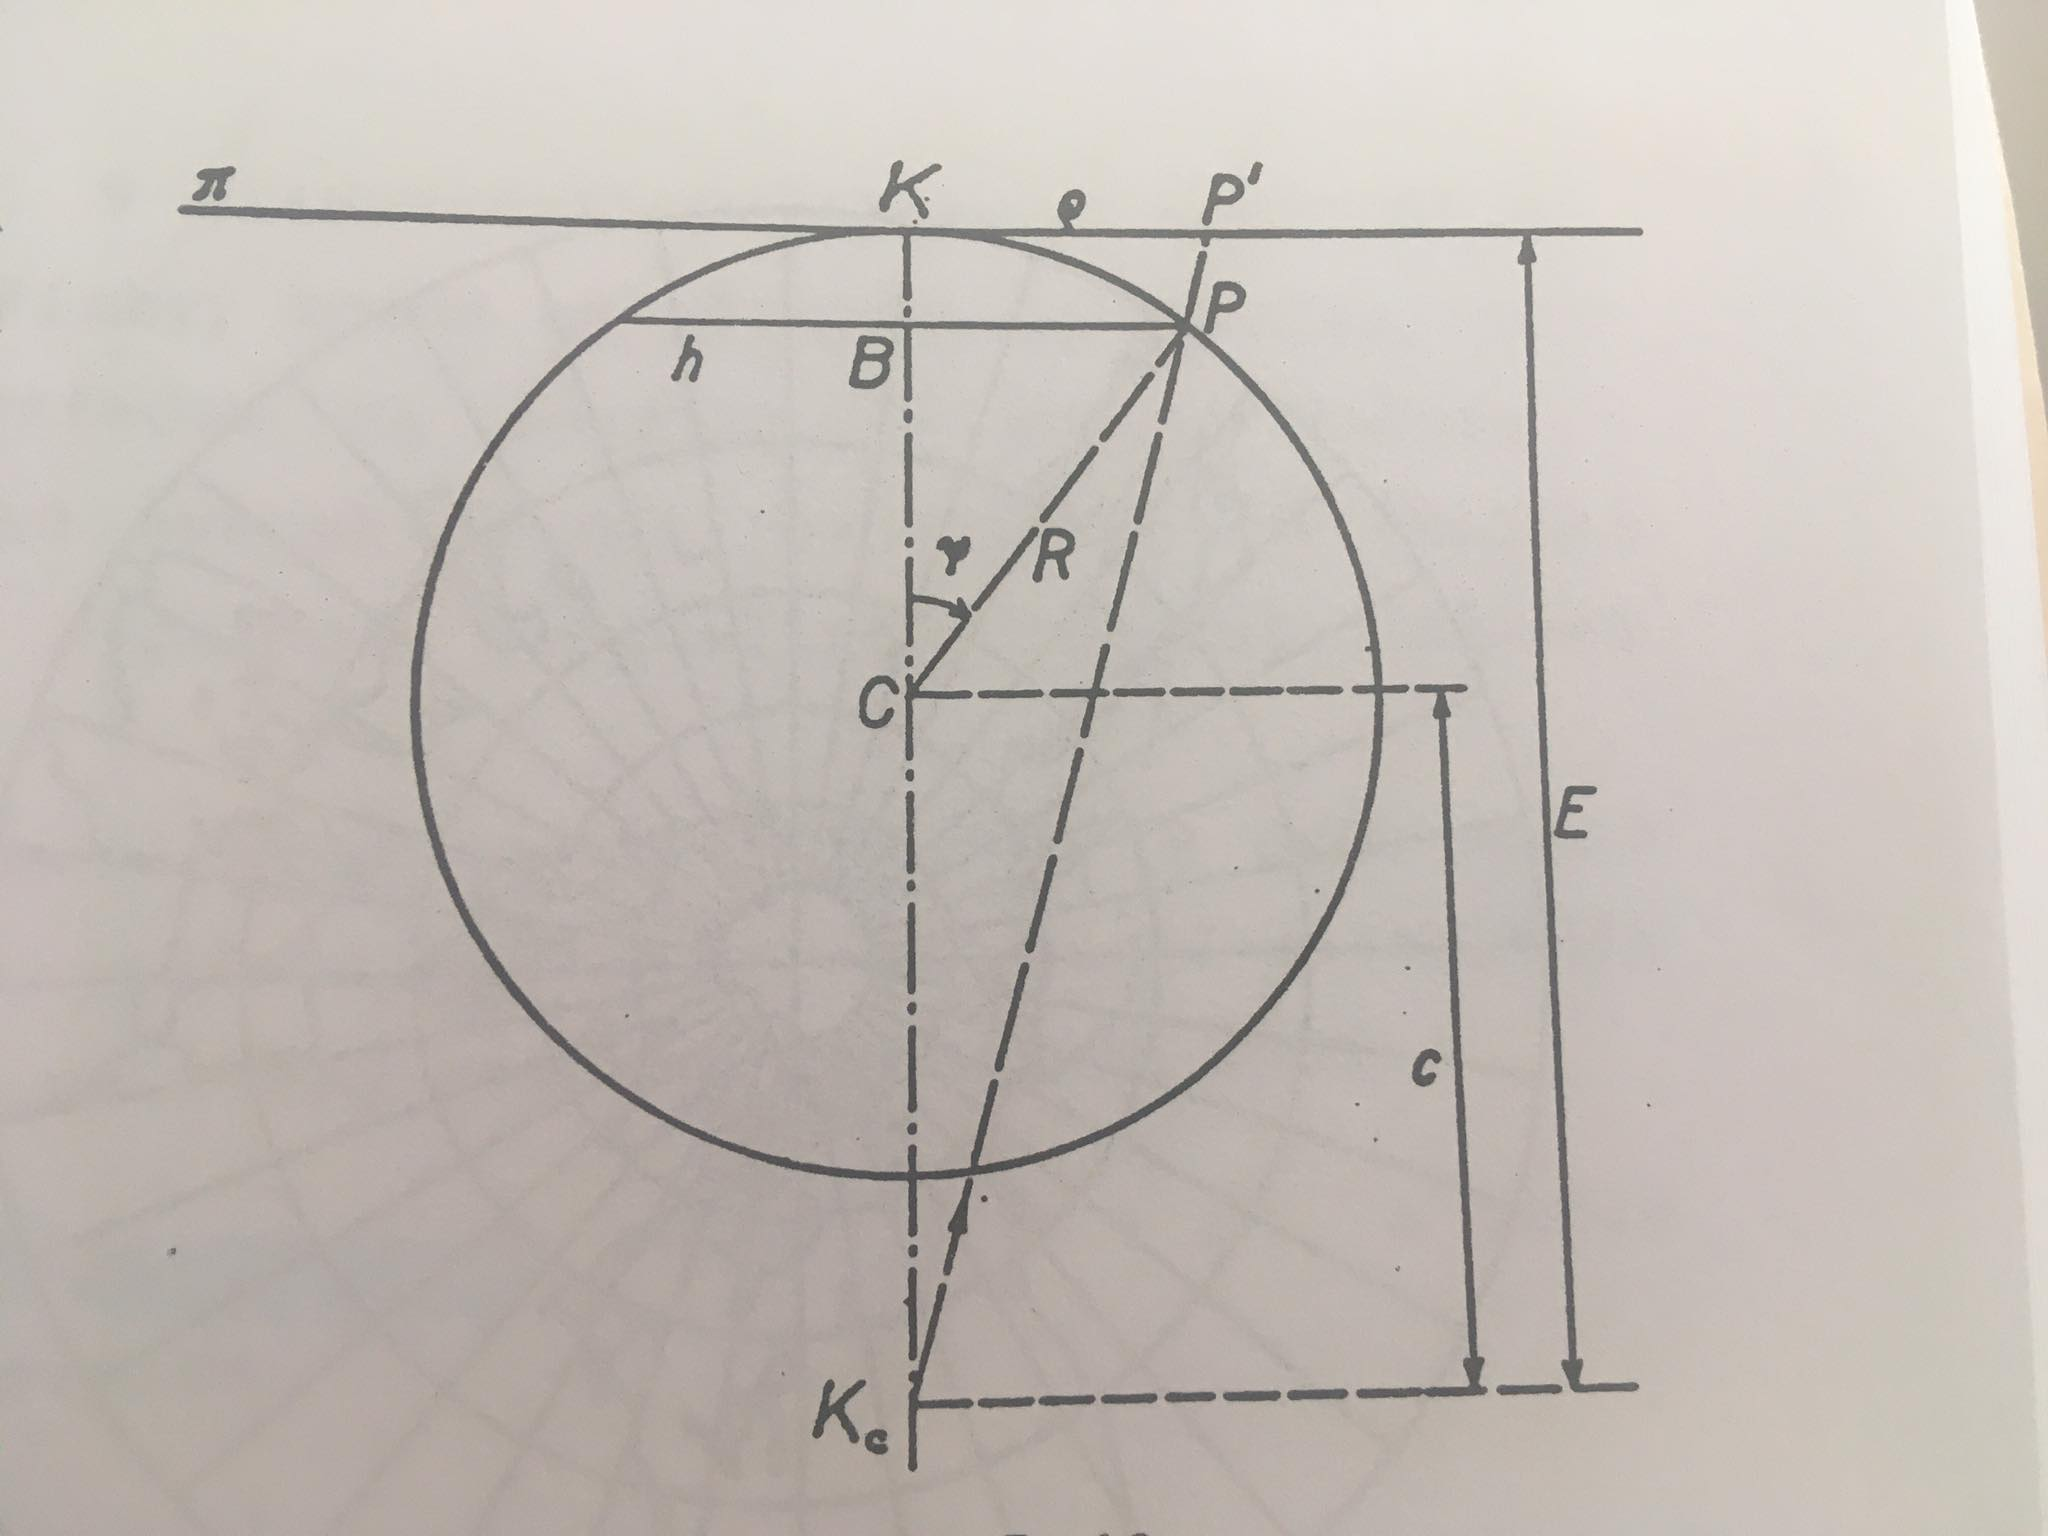
\includegraphics[width=0.5\textwidth]{FIG/azimProj.jpg}
\caption{Geometrická azimutální projekce. Obrázek je převzat z \cite{Buchar2002}.}
\label{fig:azimProj}
\end{center}
\end{figure}

Z obrázku plyne táto nerovnost
\begin{equation}
\dfrac{\rho}{R\sin{\left(\psi\right)}} = \dfrac{E}{c+R\cos{\left(\psi\right)}},
\end{equation}
kde $E = K_{c}K$ a $c = K_{c}C$, kde \textit{C} je střed koule. Takže zobrazovací rovnice azimutálních zobrazení budou

\begin{equation}
\rho = \dfrac{RE\sin{\left(\psi\right)}}{c+R\cos{\left(\psi\right)}}
\end{equation}
a
\begin{equation}
\varepsilon = \lambda.
\end{equation}

Vztahy pro výpočet pravouhlých souřadníc transformované z polárních souřadníc, resp. přímo ze zeměpisných souřadníc jsou (porovnej s \cite{stereoWolf} anebo \cite{Thomas1977},  kde je přehozené značení souřadnicových os).
\begin{equation}
X = \dfrac{RE\left(-\cos{\left(\varphi_{K}\right)}\sin{\left(\varphi\right)}+\sin{\left(\varphi_{K}\right)}\cos{\left(\varphi\right)}\cos{\left(\Delta\lambda\right)}\right)}{c+R\left( \sin{\left(\varphi_{K}\right)}\sin{\left(\varphi\right)}+\cos{\left(\varphi_{K}\right)}\cos{\left(\varphi\right)}\cos{\left(\Delta\lambda\right)} \right)},
\end{equation}
a
\begin{equation}
Y = \dfrac{RE\left(\cos{\left(\varphi\right)}\sin{\left(\Delta\lambda\right)}\right)}{c+R\left( \sin{\left(\varphi_{K}\right)}\sin{\left(\varphi\right)}+\cos{\left(\varphi_{K}\right)}\cos{\left(\varphi\right)}\cos{\left(\Delta\lambda\right)} \right)},
\end{equation}
kde $\Delta\lambda = \left(\lambda - \lambda_{K}\right)$.

Rovnice platí pro všechny azimutální projekce. Jedina neznáma konstanta \textit{c} rozhoduje výběr projekce zo sady případů, z nichž užívané jsou:
\begin{itemize}
\item gnomická projekce, při $c = 0$;
\item {\textbf{stereografická projekce}}, při $c = R$;
\item externí projekce, při $c > R$;
\item ortografická projekce, při $c = \infty$.
\end{itemize} 

Poznamenajme, že rovnice stereografické projece, která zobrazuje referenční těleso elipsoid do roviny jsou obsahem knihy \cite{Snyder1987}.

\subsection{STEREO $\rightarrow$ GEOD}.

Inverzní vzorce pro odhad zeměpisných souřadníc z pravouhlých rovinných souřadníc jsou \cite{Thomas1977} anebo \cite{stereoWolf} (pozor na přehozené značení souřadnicových os):

\begin{equation}
\varphi = \sin^{-1}{\left(\cos{\left(c\right)}\sin{\left(\varphi_{K}\right)}\dfrac{Y\sin{\left(c\right)}\cos{\left(\varphi_{K}\right)}}{\rho}\right)},
\end{equation}
a
\begin{equation}
\lambda = \lambda_{0} +  \tan^{-1}{\left(\dfrac{X\sin{\left(c\right)}}{\rho\cos{\left(\varphi_{K}\right)}\cos{\left(c\right)}-Y\sin{\left(\varphi_{K}\right)}\sin{\left(c\right)}}\right)},
\end{equation}
kde
\begin{equation}
\rho = \sqrt{X^{2} + Y^{2}}
\end{equation}
a
\begin{equation}
c = 2\tan^{-1}{\left(\dfrac{\rho}{2R}\right)}.
\end{equation}



\bibliographystyle{alpha}
\bibliography{Texty/zoznamLiteratury.bib} 

\newpage
\begin{appendices}

\section{Základní parametry zemského elipsoidu} \label{appRefEll}

\begin{table}[ht!]
\begin{tabular}{c l}

a & hlavní poloosa meridiánové elipsy \\
b & vedlejší poloosa meridiánové elipsy\\
f & zploštění (první)\\
n & zploštění (druhé)\\
e & excentricita (první)\\
$e^{'}$ & excentricita (druhá)\\
c & pólový poloměr křivosti\\
M & meridiánový poloměr křivosti\\
N & příčný poloměr křivosti\\
R & střední poloměr křivosti\\
r & poloměr rovnoběžky\\
$\varphi$ & zeměpisná šířka\\
$B_{0}^{\varphi}$ & délka oblouku meridiánu od rovníku po $\varphi$ \\
W & první geodetická funkce\\
V & druhá geodetická funkce\\
F & pomocná geodetická funce\\      
\end{tabular}
\end{table}

\begin{equation}
f = (a-b)/a.
\end{equation}

\begin{equation}
n = (a-b)/(a+b).
\end{equation}

\begin{equation}
e^{2} = (a^{2}-b^{2})/a^{2}.
\end{equation}

\begin{equation}
e^{'2} = (a^{2}-b^{2})/b^{2}.
\end{equation}

\begin{equation}
c = a^{2}/b.
\end{equation}

\begin{equation}
M = a\left(1-e^{2}\right) / W^{3}.
\end{equation}

\begin{equation}
N = a/W.
\end{equation}

\begin{equation}
R = \sqrt{M N}
\end{equation}

\begin{equation}
r = N\cos{\left(\varphi\right)}.
\end{equation}

\begin{equation}
W = \sqrt{1-e^{2}\sin^{2}{\left(\varphi\right)}}
\end{equation}

\begin{equation}
V = \sqrt{1+e^{'2}\cos^{2}{\left(\varphi\right)}}
\end{equation}

\begin{equation}
F = \sqrt{1+n\cos{\left(2\varphi\right)}+n^{2}}
\end{equation}

\section{Konstanty základních referenčních elipsoidů} \label{appRefEllConst}

\subsection{World Geodetic System 1984 (WGS84)}\label{appRefEllConstWGS84}
\begin{table}[ht!]
\begin{tabular}{c c c}
$a = 6 378 137 m$ & $b = 6 356 752,31425 m$ & $f = 0,00335 28106 64747$ \\
\end{tabular}
\end{table}

\subsection{Geodetic Reference System 1980 (GRS80)}
\begin{table}[ht!]
\begin{tabular}{c c c}
$a = 6 378 137 m$ & $b = 6 356 752,31414 m$ & $f = 0,00335 28106 81182$ \\
\end{tabular}
\end{table}

\subsection{Konstanty Krasovského elipsoidu}
\begin{table}[ht!]
\begin{tabular}{c c c}
$a = 6 378 245 m$ & $b = 6 356 863,01877 m$ & $f = 0,00335 23298 69259$ \\
\end{tabular}
\end{table}


\section{Pseudokódy implementovaných transformácii v Matlab package +Geo}

\subsection{ECEF2ENU} \label{appEcef2Enu}

\begin{algorithm}[H]
 \KwData{x, y, z, $\varphi$, $\lambda$, hel, RT, ELL}
 \KwResult{e, n, u}
 výpočet rotační matice $\mathbf{R}\left(\varphi, \lambda\right)$\;	
 \eIf{RT == elipsoid}{
  $[x_{0}, y_{0}, z_{0}] = geod2ecef(\varphi, \lambda, hel, ELL)$\;
  }{
  $[x_{0}, y_{0}, z_{0}] = sphere2ecef(\varphi, \lambda, hel^{*})$\;
 }
 Výpočet podle rovnice \ref{rov:ecef2enu22}
 \caption{Transformácia ECEF2ENU}
\end{algorithm} 

\subsection{ENU2ECEF} \label{appEnu2Ecef}

\begin{algorithm}[H]
 \KwData{e, n, u, $\varphi$, $\lambda$, hel, RT, ELL}
 \KwResult{x, y, z}
 výpočet rotační matice $\mathbf{R}\left(\varphi, \lambda\right)$\;	
 \eIf{RT == elipsoid}{
  $[x_{0}, y_{0}, z_{0}] = geod2ecef(\varphi, \lambda, hel, ELL)$\;
  }{
  $[x_{0}, y_{0}, z_{0}] = sphere2ecef(\varphi, \lambda, hel^{*})$\;
 }
 Výpočet podle rovnice \ref{rov:ecef2enu33}
 \caption{Transformácia ENU2ECEF}
\end{algorithm} 

\subsection{GEOD2ECEF} \label{appGeod2Ecef}

\begin{algorithm}[H]
 \KwData{$\varphi$, $\lambda$, h, ELL}
 \KwResult{x, y, z}
 výpočet potřebních parametrů rotačního elipsoidu (a, b, N)
 
 Výpočet podle rovnice \ref{rov:geodEcef}
 \caption{Transformácia GEOD2ECEF}
\end{algorithm} 

\subsection{ECEF2GEOD} \label{appEcef2Geod}

\begin{algorithm}[H]
 \KwData{x, y, z, ELL}
 \KwResult{$\varphi$, $\lambda$, h}
 výpočet potřebních parametrů rotačního elipsoidu (například a, e)
 
 Výpočet podle algoritmu diskutovaný např. \cite{Vermeille2011}.
 \caption{Transformácia ECEF2GEOD}
\end{algorithm} 

\section{Smerové kosíny}

\section{Elipsa chýb a Helmertová krivka}

K určeniu presnosti dvojrozmernej náhodnej veličiny je vhodné správne rozumieť chybám v rovine. Presnosť je po štatistickej stránke daná dvoma odchýlkami s normálnym rozdelením. Presnosť je teda v konkrétnom súradnom systéme, napr. v systéme pravouhlých kartézianských súradníc x, y, definovaná tzv. kovariančnou maticou v tvare:

\begin{equation}\label{rov:el1}
\mathbf{Q}=
\begin{pmatrix} 
\sigma_x             & \sigma_{x}\sigma_{y}  \\  
\sigma_{x}\sigma_{y} & \sigma_{y} 
\end{pmatrix}, 
\end{equation}

kde 

\begin{itemize}
\item $\sigma_{x}$ je druhá odmocnina rozptylu veličiny x a reprezentuje charakteristiku presnosti tejto veličiny,
\item $\sigma_{y}$ je druhá odmocnina rozptylu veličiny y a rovnako reprezentuje charakteristiku presnosti tejto veličiny,
\item $\sigma_{x}\sigma_{y}$ je kovariancia medzi parametrami x a y (v literatúre $\sigma_{x, y}$ alebo $Cov_{x, y}$).
\end{itemize}
  
Plochu elipsy, ktorú odvodíme z informácií z danej kovariančnej matice \ref{rov:el1}, opisujú tri základné veličiny: a) smerodajná odchýlka v smere hlavnej polosi $\sigma_a$, b) smerodajná odchýlka v smere vedľajšej poloosi $\sigma_b$ a c) uhol natočenia celej plochy $\vartheta$. Tieto kolmé smerodajné odchýlky spoločne s uhlom natočenia je možné odvodiť viacerými spôsobmi. Sledujúc prácu \cite{Hampacher2003}, vychádzajme z predpokladu, že hustota pravdepodobnosti je definovaná predpisom:

\begin{equation}
\varphi(x, y) = \dfrac{1}{2 \pi \sigma_{x} \sigma_{y} \sqrt{(1-\rho^2)} }  \exp\left\lbrace \dfrac{-1}{2 \left( 1- \rho^2 \right)} \left[ \frac{x^2}{\sigma_{x}^{2}} + \frac{y^2}{\sigma_{y}^{2}} -2 \rho \frac{xy}{\sigma_{x} \sigma_{y}} \right] \right\rbrace,
\end{equation}
kde

\begin{itemize}
\item  $\rho$ je koeficient korelácie.
\end{itemize}
V prípade, ak veličiny x a y sú nezávislé, koeficient korelácie je nulový. Naopak, ak veličiny sú korelované dostaneme rovnicu elipsy v tvare:

\begin{equation}\label{rov:oko}
 \dfrac{1}{1-\rho^2} \left( \dfrac{x^2}{\sigma_{x}^{2}} + \dfrac{y^2}{\sigma_{y}^{2}} -2 \rho \frac{xy}{\sigma_{x} \sigma_{y}} \right)  = t^2,
\end{equation}
kde \textit{t} je normovaná veľkosť dvojrozmernej chyby.

Ďalej bez ďalšieho odvodenia, dôjdeme k výsledku, podľa ktorého veľkosť hlavnej osi elipsy (smerodajnej odchýlky $\sigma_a$) je:

\begin{equation}\label{rov:sigA}
\sigma_a = \left\lbrace \dfrac{1}{2} \left[ \sigma_x^2 + \sigma_y^2 + \sqrt{\left(\sigma_{x}^{2}-\sigma_{y}^{2}\right)^2 + 4\rho\sigma_{x}^2\sigma_{y}^2} \right]\right\rbrace^{\dfrac{1}{2}},
\end{equation}
a veľkosť vedľajšej osi elipsy
\begin{equation}\label{rov:sigB}
\sigma_b = \left\lbrace \dfrac{1}{2} \left[ \sigma_x^2 + \sigma_y^2 - \sqrt{\left(\sigma_{x}^{2}-\sigma_{y}^{2}\right)^2 + 4\rho\sigma_{x}^2\sigma_{y}^2} \right]\right\rbrace^{\dfrac{1}{2}}.
\end{equation}

Natočenie elipsy môžeme opísať vzorcom

\begin{equation}\label{rov:nat}
\tan{\left(2\vartheta\right)} = 2\rho\dfrac{\sigma_{x}\sigma_{y}}{\sigma_{x}^2 - \sigma_{y}^2}.
\end{equation}

K rovnakému výsledku sa dá dôjsť spektrálnym rozkladom kovariančnej matice $\mathbf{Q}$ (náčrt rozkladu a odvodenia je v prílohe).

Význam veličín $\sigma_a$, $\sigma_b$ a $\vartheta$ sa často zobrazuje ako elipsa chýb a je to krivka, ktorá spojuje body s rovnakou hustotou pravdepodobnosti. To znamená, že hlavná poloosa, ktorá je odvodená od rovnice \ref{rov:sigA} je od pôvodnej súradnej sústavy odklonená o uhol opísaný rovnicou \ref{rov:nat} a že rovnica \ref{rov:oko} obecne definuje okolie skutočnej polohy veličiny, v ktorom by sa teoreticky malo vyskytovať isté percento možných hodnôt.

Z uvedeného rozloženia chýb v rovine je možné, opäť s istou pravdepodobnosťou, odvodiť aj neistotu určenia polohy bodu v ľubovoľnom smere. Krivka, ktorá spojuje presnosť pre všetky smery sa nazýva \textit{Helmertová krivka}.

Pre odhad presnosti použijeme zákon hromadenia stredných chýb. Všeobecný zápis zákona je tento \cite{Hampacher2003}:

\begin{equation}
m_f^2 = \mathbf{f}^T\mathbf{Q}\mathbf{f},
\end{equation}
kde
\begin{itemize}
\item $\mathbf{f}$ je vektor smerových kosínov,
\item $\mathbf{Q}$ je hore definovaná kovariančná matica a
\item $m_f^2$ je prievodič bodu Helmertovej krivky, t.j. veľkosť rozptylu v smere danej priamky $\sqrt{x^2+y^2}$.
\end{itemize}

Bez odvodenia, rovnica Helmertovej krivky je %\cite{Kocandrlova2000}, \cite{Hampacher2003}.

%[Hampacher2003] Hampacher M., (2003). Elipsa chyb a Helmertova křivka trochu jinak. Geodetický a kartografický obzor, 49/91, číslo 10.
%[Kocandrlova2000] Kočandrlova M., (2000). Helmertová křivka. Geodetický a kartografický obzor 46/88, číslo 6.

Jej vyjadrenie je
\begin{equation}
 \left( x^2 + y^2\right)^2 = x^2\sigma_x^2 + y^2\sigma_y^2 + 2\rho \sigma_x \sigma_y xy.
\end{equation}

\newpage
\subsection{Príklad zobrazenia elipsy chýb a Helmertovej krivky}

Prvý príklad poukazuje na stav v ktorom kovariančná matica vyjadruje nezávislé veličiny.

Jej vyjadrenie je: 

\begin{equation}
\mathbf{Q}=
\begin{pmatrix}
 2 & 0  \\
 0 & 5
\end{pmatrix}.
\end{equation}

\begin{figure}[ht!]
\begin{center}
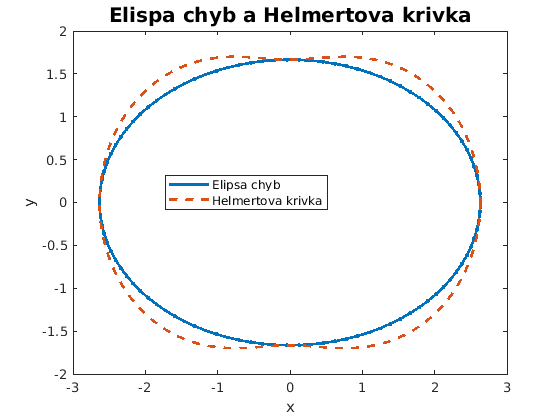
\includegraphics[width=0.5\textwidth]{FIG/s2-5cov0-0.png}
\end{center}
\caption{Zobrazenie elipsy chýb a Helmertovej krivky. Kovariancia je 0.0.}
\end{figure}

Druhý príklad poukazuje na stav v ktorom kovariančná matica vyjadruje závislé veličiny.

Jej vyjadrenie je: 

\begin{equation}
\mathbf{Q}=
\begin{pmatrix} 
  2 & 1.5  \\
1.5 & 5 
\end{pmatrix}.
\end{equation}

\begin{figure}[ht!]
\begin{center}
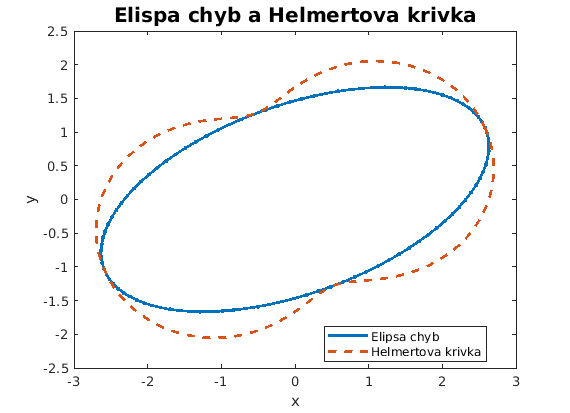
\includegraphics[width=0.5\textwidth]{FIG/s2-5cov1.5-1.5.png}
\end{center}
\caption{Zobrazenie elipsy chýb a Helmertovej krivky. Kovariancia je 1.5.}
\end{figure}

Posledný príklad obshahuje stav transformácie kovariančnej matice zo systému ECEF do systému ENU pravouhlých súradníc. Scatter ploty pod diagonálou obsahujú aj porovnanie elíps chýb a Helmertových kriviek. Z príkladu je pozorovateľné, že ak sa druhé odmocniny rozptylov veličín približne rovnajú a veličiny nie sú korelované (v príklade takými veličinami sú súradnice N (north) a U (up) v korelácii so súradnicou E (east)) tak polygóny elipsy chýb a Helmertových kriviek sa veľmi zhodujú. Naopak, ak sú data korelované (z príkladu pozorujeme závislosť veličín N a U), vidíme neistoty určenia polôh bodov v danom smere značne odlišné (bola uvažovaná $90\%$ hladina významnosti).

\begin{figure}
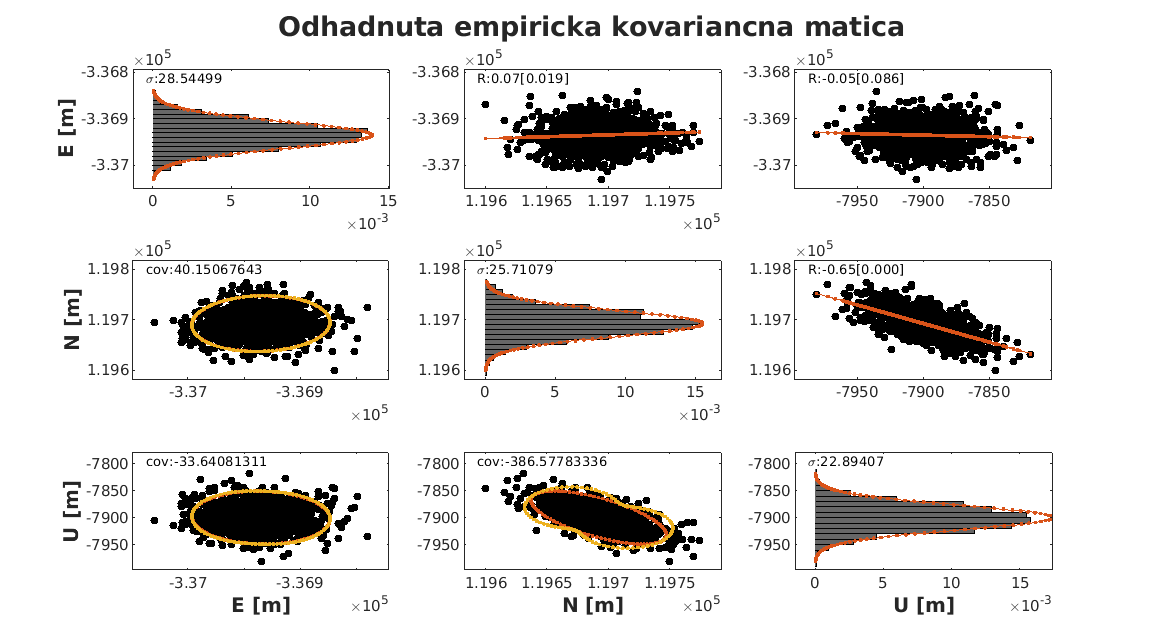
\includegraphics[width=1.0\textwidth]{FIG/ecef2enu.png}
\caption{Transformácia suradníc zo súradného systému ECEF do systému ENU.}
\end{figure}

\section{Vlastné čísla a vlastné vektory}

\subsection{Spektrálny rozklad štvorcovej matice}

Bez dokazovania.

Nech $\mathbf{Q}$ je štvorcová matica s rozmerom $n\times n$. Potom spektrálnym rozkladom takejto matice je rozklad matice na vlastné čísla a vlastné vektory a platí:

\begin{equation}
\mathbf{Q} = \sum_{i=1}^{n}\lambda_{i}\mathbf{f}_{i}\mathbf{f}_{i}^{T},
\end{equation}

kde
\begin{itemize}
\item $\mathbf{f}_{i}\mathbf{f}_{i}^{T}$ sú vlastné vektory a
\item $\lambda_{i}$ sú vlastné čísla.
\end{itemize}

Ak pre skalár $\lambda$ a pre vektor $\mathbf{f}$, ktorý je nenulový platí

\begin{equation}
\mathbf{Af} = \lambda\mathbf{f}
\end{equation}

potom $\lambda$ je vlastné číslo matice $\mathbf{Q}$ a vektor $\mathbf{f}$ je vlastný vektor matice $\mathbf{Q}$ a príslušný vlastnému číslu $\lambda$.

Platí, že vlastný vektor matice je príslušný jednej vlastnej hodnote tejto matice. Vlastné čísla matice s rozmerom napr. $2\times 2$ získame riešením rovnice:

\begin{equation}\label{rov:spec1}
Det\left(\mathbf{Q} - \lambda\mathbf{I}\right) = \lambda^2 - Tr(\mathbf{Q})\lambda + Det(\mathbf{Q}) = 0
\end{equation}
a potom

\begin{equation}\label{rov:spec2}
\begin{vmatrix} 
q_{11} - \lambda & q_{12}  \\ 
 q_{21} & q_{22} - \lambda 
 \end{vmatrix} = 0.
\end{equation}

Je to nutná a postačujúca podmienka pre existenciu vlastného vektoru matice $\mathbf{Q}$ príslušného $\lambda$.

\subsection{Návrh odvodenia prvkov elipsy chýb za pomoci spektrálneho rozkladu štvorcovej matice}

Majme kovariančnú maticu $\mathbf{Q}$ v tvare,

\begin{equation}
\mathbf{Q}=
\begin{pmatrix} 
\sigma_x^2 & \rho\sigma_{x} \sigma_{y}  \\ 
\rho\sigma_{x} \sigma_{y} & \sigma_{y}^2 
\end{pmatrix}.
\end{equation}

Podľa \ref{rov:spec1} a \ref{rov:spec2} dostaneme

\begin{equation}
Det(\mathbf{Q } - \lambda\mathbf{I})  = 0
\end{equation}

a potom

\begin{equation}
\left(\sigma_x^2 - \lambda\right)\left(\sigma_y^2 - \lambda\right) - \rho^2\sigma_x^2\sigma_y^2 = 0.
\end{equation}

Po vyriešení,

\begin{eqnarray}
 \sigma_a = \sqrt{\lambda_1}  &=& \left\lbrace \dfrac{1}{2} \left[ \sigma_x^2 + \sigma_y^2 + \sqrt{\left(\sigma_x^2-\sigma_y^2\right)^2 +4\rho\sigma_{x}^2\sigma_{y}^2} \right]\right\rbrace^{\frac{1}{2}} , \\
\sigma_b = \sqrt{\lambda_2} &=& \left\lbrace \dfrac{1}{2} \left[ \sigma_x^2 + \sigma_y^2 - \sqrt{\left(\sigma_x^2-\sigma_y^2\right)^2 +4\rho\sigma_{x}^2\sigma_{y}^2} \right]\right\rbrace^{\frac{1}{2}} .
\end{eqnarray}

 
\section{Zákon hromadenia chýb - Propagation low}



\section{Zobrazení elipsoidu na kouli za podmínky zachování úhlů (konformní zobrazení)}

Poznámky pocházejí z předášek \cite{Cajthaml2014}.

\begin{itemize}
\item Musí být splněny podmínky konformity
\begin{equation}
m_{r} = m_{p},\ \ p = 0.
\end{equation}
Při odvození stačí uvažovat první podmínku. Tá druhá je splněna tím, že zeměpisná siť se zobrazuje jako zeměpisná síť (viz přednáška 3 \cite{Cajthaml2014}).
\begin{equation}
\dfrac{R dU}{Md\varphi} = \dfrac{R\cos{\left(U\right)}dV}{N\cos{\left(\varphi\right)}d\lambda}.
\end{equation}
\item Vzhledem k tomu, že intervaly zeměpisné délky musí být symetrické, pak
\begin{equation}
dV = \alpha d\lambda.
\end{equation}
\item Výslední zobrazovací rovnice (bez odvození) jsou:
\begin{equation}
\tan{\left(\dfrac{U}{2}+45^{\circ}\right)} = \dfrac{1}{k}\left[\tan{\left(\dfrac{\varphi}{2}+45^{\circ}\right)}  \left(\dfrac{1-e\sin{\left(\varphi\right)}}{1+e\sin{\left(\varphi\right)}} \right)^{e/2}  \right]^{\alpha}
\end{equation}
\begin{equation}
V = \alpha\lambda.
\end{equation}
\end{itemize}
\subsection*{Zkreslení}
Pro zkreslení platí
\begin{equation}
m = \dfrac{\alpha R \cos{\left(U\right)}}{N\cos{\left(\varphi\right)}},
\end{equation}
\begin{equation}
P = m^{2},
\end{equation}
a
\begin{equation}
\Delta\omega = 0.
\end{equation}

\subsection*{Volba konstant zobrazení}

Pokud má být zobrazení souvislé (celý elipsoid na celou kouli), pak
\begin{equation}
\alpha = 1,
\end{equation}

\begin{equation}
k = 1,
\end{equation}
a
\begin{equation}
R = a.
\end{equation}
Pokud má být zobrazené jenom dílčí území mezi  $\varphi_{J}$ a $\varphi_{S}$, pak (Gaussův způsob):
\begin{itemize}
\item zvolí se základní rovnoběžka $\varphi_{0}$ (uprostřed území), která zůstane nezkreslená, t.j.
\begin{equation}
m_{0} = 1,
\end{equation}
\item pomocí Taylorova rozvoje se vzorec pro délkové zkreslení odvodí do tvaru
\begin{equation}
m = f\left(\varphi\right) = f\left(\varphi_{0}+\Delta\varphi\right) = f\left(\varphi_{0}\right) + \Delta\varphi\dfrac{dm}{d\varphi} + \Delta\varphi^{2}\dfrac{d^{2}m}{2! d^{2}\varphi} + \cdots 
\end{equation}
\item Aby délkové zkreslení bylo co nejmenší, zvolí se podmínky
\begin{equation}
m_{0} = 1,
\end{equation}
\begin{equation}
\dfrac{dm}{d\varphi} = 0, 
\end{equation}
a
\begin{equation}
\dfrac{d^{2}m}{d^{2}\varphi} = 0.
\end{equation}
\item Z předchozích podmínek (bez odvození), pro hledané konstanty dostaneme týto vztahy
\begin{equation}
\alpha^{2} = 1+\dfrac{e^{2}\cos^{4}{\left(\varphi_{0}\right)}}{1-e^{2}},
\end{equation}
přičemž
\begin{equation}
\sin{\left(\varphi_{0}\right)} = \alpha\sin{\left(U_{0}\right)}.
\end{equation}
A dále, 
\begin{equation}
k = \dfrac{\tan^{\alpha}{\left(\dfrac{\varphi_{0}}{2}+45^{\circ}\right)}\left(\dfrac{1-e\sin{\left(\varphi_{0}\right)}}{1+e\sin{\left(\varphi_{0}\right)}}\right)^{\dfrac{\alpha e}{2}}}{\tan{\left(\dfrac{U_{0}}{2}+45^{\circ}\right)}},
\end{equation}
a
\begin{equation}
R = \sqrt{M_{0}N_{0}}.
\end{equation}
\end{itemize} 

\section{Meridánová konvergence - poznámky}

Při převodu zeměpisných (např. elipsoidických) souřadníc do zobrazovací roviny některého zobrazovacího systému by mohla platiť táto schéma převodu (viz nasledující obrázek):

\begin{figure}[ht!]
\begin{center}
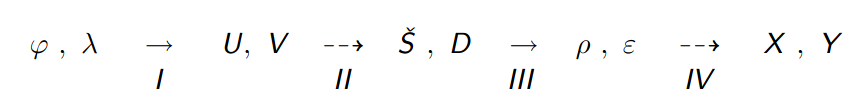
\includegraphics[width=1\textwidth]{FIG/schema}
\caption{Obecná schéma možného převodu elipsoidicých souřadníc do systému zobrazovacích souřadníc.}
\label{fig:schema}
\end{center}
\end{figure}


\begin{enumerate}
\item Blok \textbf{I} představuje konformní zobrazení elipsoidických souřadníc na kouli (například Gaussovým způsobem).
\item Blok \textbf{II} jsou zeměpisne sférické spuřadnice převedeny na kartografické souřadnice a to vzhledem k zvolenému kartografckému pólu.
\item  Blok \textbf{III} obsahuje konformní zobrazení kartografických souřadníc z koule na zvolenou zobrazovací plochu (kužel, válec, rovina).
\item Blok \textbf{IV} obsahuje výpočet pravouhlých souřadníc z polárních souřadníc.
\end{enumerate}

Meridiánová konvergence je úhel mezi zemským poledníkem a rovnoběžkou rovnoběžnou s osou Y (X - v závislosti na tom, jak je souřadnicový sýstém zobrazovací roviny definován). 

Speciálne pro stereografickou projekci, pokud by byla stereografická projekce v normálni poloze (na pólu) tak meridiánová konvergence se rovná přímo zeměpisné délce. Pokud stereografická projekce bude definováná v obecné poloze, postup odhadu meridánové konvergence by mohl být tento: 

\begin{itemize}
\item Zeměpisné souřadnice U, V pomocí nasledujících vztahů převedeme na kartografické souřadnice, s, d (platí pro převod na koulové ploše)
\begin{equation}
\sin{\left(s\right)} = \sin{\left(U_{k}\right)}\sin{\left(U\right)}+\cos{\left(U_{k}\right)}\cos{\left(U\right)}\cos{\left(\Delta V\right)}
\end{equation}
\begin{equation}
\sin{\left(d\right)}=\dfrac{\sin{\left(\Delta V\right)}\cos{\left(U\right)}}{\cos{\left(s\right)}}.
\end{equation}
\item Nasleduje výpočet souřadnice $\varepsilon$, například pomocí této zobrazovací rovnice
\begin{equation}
\varepsilon = nD,
\end{equation}
kde D je zeměpisná délka na kouli a n je konstanta zobrazení.
\item U vrcholu P sféfirckého trojuholníku se musí vypočítat vnitří úhel $\xi$
\begin{equation}
\sin{\left(\xi\right)} = \dfrac{\cos{\left(U_{k}\right)}\sin{\left(D\right)}}{\sin{\left(U\right)}}.
\end{equation}
\item Potom meridiánová konvergence se vypočte pomocí rovnice $C = \varepsilon - \xi$. Platí také přibližný vzorec
\begin{equation}
C = 0.008257 Y + 2.373\dfrac{Y}{X}\ [km],
\end{equation}
kde Y a X jsou pravouhlé souřadnice, přičemž X je obrazem základního poledníku a Y je kolmá na X.
\end{itemize}

\end{appendices}


\end{document}
